% Options for packages loaded elsewhere
\PassOptionsToPackage{unicode}{hyperref}
\PassOptionsToPackage{hyphens}{url}
%
\documentclass[
]{book}
\title{Data Science: A First Introduction}
\author{Tiffany-Anne Timbers \and Trevor Campbell \and Melissa Lee}
\date{2021-10-03}

\usepackage{amsmath,amssymb}
\usepackage{lmodern}
\usepackage{iftex}
\ifPDFTeX
  \usepackage[T1]{fontenc}
  \usepackage[utf8]{inputenc}
  \usepackage{textcomp} % provide euro and other symbols
\else % if luatex or xetex
  \usepackage{unicode-math}
  \defaultfontfeatures{Scale=MatchLowercase}
  \defaultfontfeatures[\rmfamily]{Ligatures=TeX,Scale=1}
\fi
% Use upquote if available, for straight quotes in verbatim environments
\IfFileExists{upquote.sty}{\usepackage{upquote}}{}
\IfFileExists{microtype.sty}{% use microtype if available
  \usepackage[]{microtype}
  \UseMicrotypeSet[protrusion]{basicmath} % disable protrusion for tt fonts
}{}
\makeatletter
\@ifundefined{KOMAClassName}{% if non-KOMA class
  \IfFileExists{parskip.sty}{%
    \usepackage{parskip}
  }{% else
    \setlength{\parindent}{0pt}
    \setlength{\parskip}{6pt plus 2pt minus 1pt}}
}{% if KOMA class
  \KOMAoptions{parskip=half}}
\makeatother
\usepackage{xcolor}
\IfFileExists{xurl.sty}{\usepackage{xurl}}{} % add URL line breaks if available
\IfFileExists{bookmark.sty}{\usepackage{bookmark}}{\usepackage{hyperref}}
\hypersetup{
  pdftitle={Data Science: A First Introduction},
  pdfauthor={Tiffany-Anne Timbers; Trevor Campbell; Melissa Lee},
  hidelinks,
  pdfcreator={LaTeX via pandoc}}
\urlstyle{same} % disable monospaced font for URLs
\usepackage{color}
\usepackage{fancyvrb}
\newcommand{\VerbBar}{|}
\newcommand{\VERB}{\Verb[commandchars=\\\{\}]}
\DefineVerbatimEnvironment{Highlighting}{Verbatim}{commandchars=\\\{\}}
% Add ',fontsize=\small' for more characters per line
\usepackage{framed}
\definecolor{shadecolor}{RGB}{248,248,248}
\newenvironment{Shaded}{\begin{snugshade}}{\end{snugshade}}
\newcommand{\AlertTok}[1]{\textcolor[rgb]{0.33,0.33,0.33}{#1}}
\newcommand{\AnnotationTok}[1]{\textcolor[rgb]{0.37,0.37,0.37}{\textbf{\textit{#1}}}}
\newcommand{\AttributeTok}[1]{\textcolor[rgb]{0.61,0.61,0.61}{#1}}
\newcommand{\BaseNTok}[1]{\textcolor[rgb]{0.06,0.06,0.06}{#1}}
\newcommand{\BuiltInTok}[1]{#1}
\newcommand{\CharTok}[1]{\textcolor[rgb]{0.5,0.5,0.5}{#1}}
\newcommand{\CommentTok}[1]{\textcolor[rgb]{0.37,0.37,0.37}{\textit{#1}}}
\newcommand{\CommentVarTok}[1]{\textcolor[rgb]{0.37,0.37,0.37}{\textbf{\textit{#1}}}}
\newcommand{\ConstantTok}[1]{\textcolor[rgb]{0,0,0}{#1}}
\newcommand{\ControlFlowTok}[1]{\textcolor[rgb]{0.27,0.27,0.27}{\textbf{#1}}}
\newcommand{\DataTypeTok}[1]{\textcolor[rgb]{0.27,0.27,0.27}{#1}}
\newcommand{\DecValTok}[1]{\textcolor[rgb]{0.06,0.06,0.06}{#1}}
\newcommand{\DocumentationTok}[1]{\textcolor[rgb]{0.37,0.37,0.37}{\textbf{\textit{#1}}}}
\newcommand{\ErrorTok}[1]{\textcolor[rgb]{0.14,0.14,0.14}{\textbf{#1}}}
\newcommand{\ExtensionTok}[1]{#1}
\newcommand{\FloatTok}[1]{\textcolor[rgb]{0.06,0.06,0.06}{#1}}
\newcommand{\FunctionTok}[1]{\textcolor[rgb]{0,0,0}{#1}}
\newcommand{\ImportTok}[1]{#1}
\newcommand{\InformationTok}[1]{\textcolor[rgb]{0.37,0.37,0.37}{\textbf{\textit{#1}}}}
\newcommand{\KeywordTok}[1]{\textcolor[rgb]{0.27,0.27,0.27}{\textbf{#1}}}
\newcommand{\NormalTok}[1]{#1}
\newcommand{\OperatorTok}[1]{\textcolor[rgb]{0.43,0.43,0.43}{\textbf{#1}}}
\newcommand{\OtherTok}[1]{\textcolor[rgb]{0.37,0.37,0.37}{#1}}
\newcommand{\PreprocessorTok}[1]{\textcolor[rgb]{0.37,0.37,0.37}{\textit{#1}}}
\newcommand{\RegionMarkerTok}[1]{#1}
\newcommand{\SpecialCharTok}[1]{\textcolor[rgb]{0,0,0}{#1}}
\newcommand{\SpecialStringTok}[1]{\textcolor[rgb]{0.5,0.5,0.5}{#1}}
\newcommand{\StringTok}[1]{\textcolor[rgb]{0.5,0.5,0.5}{#1}}
\newcommand{\VariableTok}[1]{\textcolor[rgb]{0,0,0}{#1}}
\newcommand{\VerbatimStringTok}[1]{\textcolor[rgb]{0.5,0.5,0.5}{#1}}
\newcommand{\WarningTok}[1]{\textcolor[rgb]{0.37,0.37,0.37}{\textbf{\textit{#1}}}}
\usepackage{longtable,booktabs,array}
\usepackage{calc} % for calculating minipage widths
% Correct order of tables after \paragraph or \subparagraph
\usepackage{etoolbox}
\makeatletter
\patchcmd\longtable{\par}{\if@noskipsec\mbox{}\fi\par}{}{}
\makeatother
% Allow footnotes in longtable head/foot
\IfFileExists{footnotehyper.sty}{\usepackage{footnotehyper}}{\usepackage{footnote}}
\makesavenoteenv{longtable}
\usepackage{graphicx}
\makeatletter
\def\maxwidth{\ifdim\Gin@nat@width>\linewidth\linewidth\else\Gin@nat@width\fi}
\def\maxheight{\ifdim\Gin@nat@height>\textheight\textheight\else\Gin@nat@height\fi}
\makeatother
% Scale images if necessary, so that they will not overflow the page
% margins by default, and it is still possible to overwrite the defaults
% using explicit options in \includegraphics[width, height, ...]{}
\setkeys{Gin}{width=\maxwidth,height=\maxheight,keepaspectratio}
% Set default figure placement to htbp
\makeatletter
\def\fps@figure{htbp}
\makeatother
\setlength{\emergencystretch}{3em} % prevent overfull lines
\providecommand{\tightlist}{%
  \setlength{\itemsep}{0pt}\setlength{\parskip}{0pt}}
\setcounter{secnumdepth}{5}
\usepackage{booktabs}
\usepackage{amsthm}
\usepackage{makeidx}
\makeindex
\makeatletter
\def\thm@space@setup{%
  \thm@preskip=8pt plus 2pt minus 4pt
  \thm@postskip=\thm@preskip
}
\makeatother
\ifLuaTeX
  \usepackage{selnolig}  % disable illegal ligatures
\fi
\usepackage[]{natbib}
\bibliographystyle{apalike}

\begin{document}
\maketitle

% you may need to leave a few empty pages before the dedication page

%\cleardoublepage\newpage\thispagestyle{empty}\null
%\cleardoublepage\newpage\thispagestyle{empty}\null
%\cleardoublepage\newpage
\thispagestyle{empty}

\begin{center}
To you, the Reader.

Never stop learning. You are capable of anything.
%\includegraphics{images/dedication.pdf}
\end{center}

\setlength{\abovedisplayskip}{-5pt}
\setlength{\abovedisplayshortskip}{-5pt}

{
\setcounter{tocdepth}{2}
\tableofcontents
}
\hypertarget{preface}{%
\chapter*{Preface}\label{preface}}


This textbook aims to be an approachable introduction to the world of data science.
In this book, we define \textbf{data science} \index{data science!definition} as the process of generating
insight from data through \textbf{reproducible} \index{reproducible} and \textbf{auditable} \index{auditable} processes.
If you analyze some data and give your analysis to a friend or colleague, they should
be able to re-run the analysis from start to finish and get the same result you did (\emph{reproducibility}).
They should also be able to see and understand all the steps in the analysis, as well as the history of how
the analysis developed (\emph{auditability}). Creating reproducible and auditable
analyses allows both yourself and others to easily double-check and validate your work.

At a high level, in this book, you will learn how to

\begin{enumerate}
\def\labelenumi{(\arabic{enumi})}
\tightlist
\item
  identify common problems in data science, and
\item
  solve those problems with reproducible and auditable workflows.
\end{enumerate}

Figure \ref{fig:img-chapter-overview} summarizes what you will learn in each chapter
of this book.
Throughout, you will learn how to use the R programming language \citep{Rlanguage} to perform
all the tasks associated with data analysis. You will
spend the first four chapters learning how to use R to load, clean, wrangle
(i.e., restructure the data into a usable format) and visualize data
while answering descriptive and exploratory data analysis questions. In the next
six chapters you will learn how to answer predictive, exploratory and inferential
data analysis questions with common methods in data science, including
classification, regression, clustering and estimation.
In the final chapters
(\ref{getting-started-with-jupyter} - \ref{move-to-your-own-machine}),
you will learn how to combine R code, formatted text, and images
in a single coherent document with Jupyter, use version control for
collaboration, and install and configure the software needed for data science
on your own computer. If you are reading this book as part of a course that you are
taking, the instructor may have set up all of these tools already for you; in this
case you can continue on through the book reading the chapters in order.
But if you are reading this independently, you may want to jump to these last three chapters
early before going on to make sure your computer is set up in such a way that you can
try out the example code that we include throughout the book.

\begin{figure}
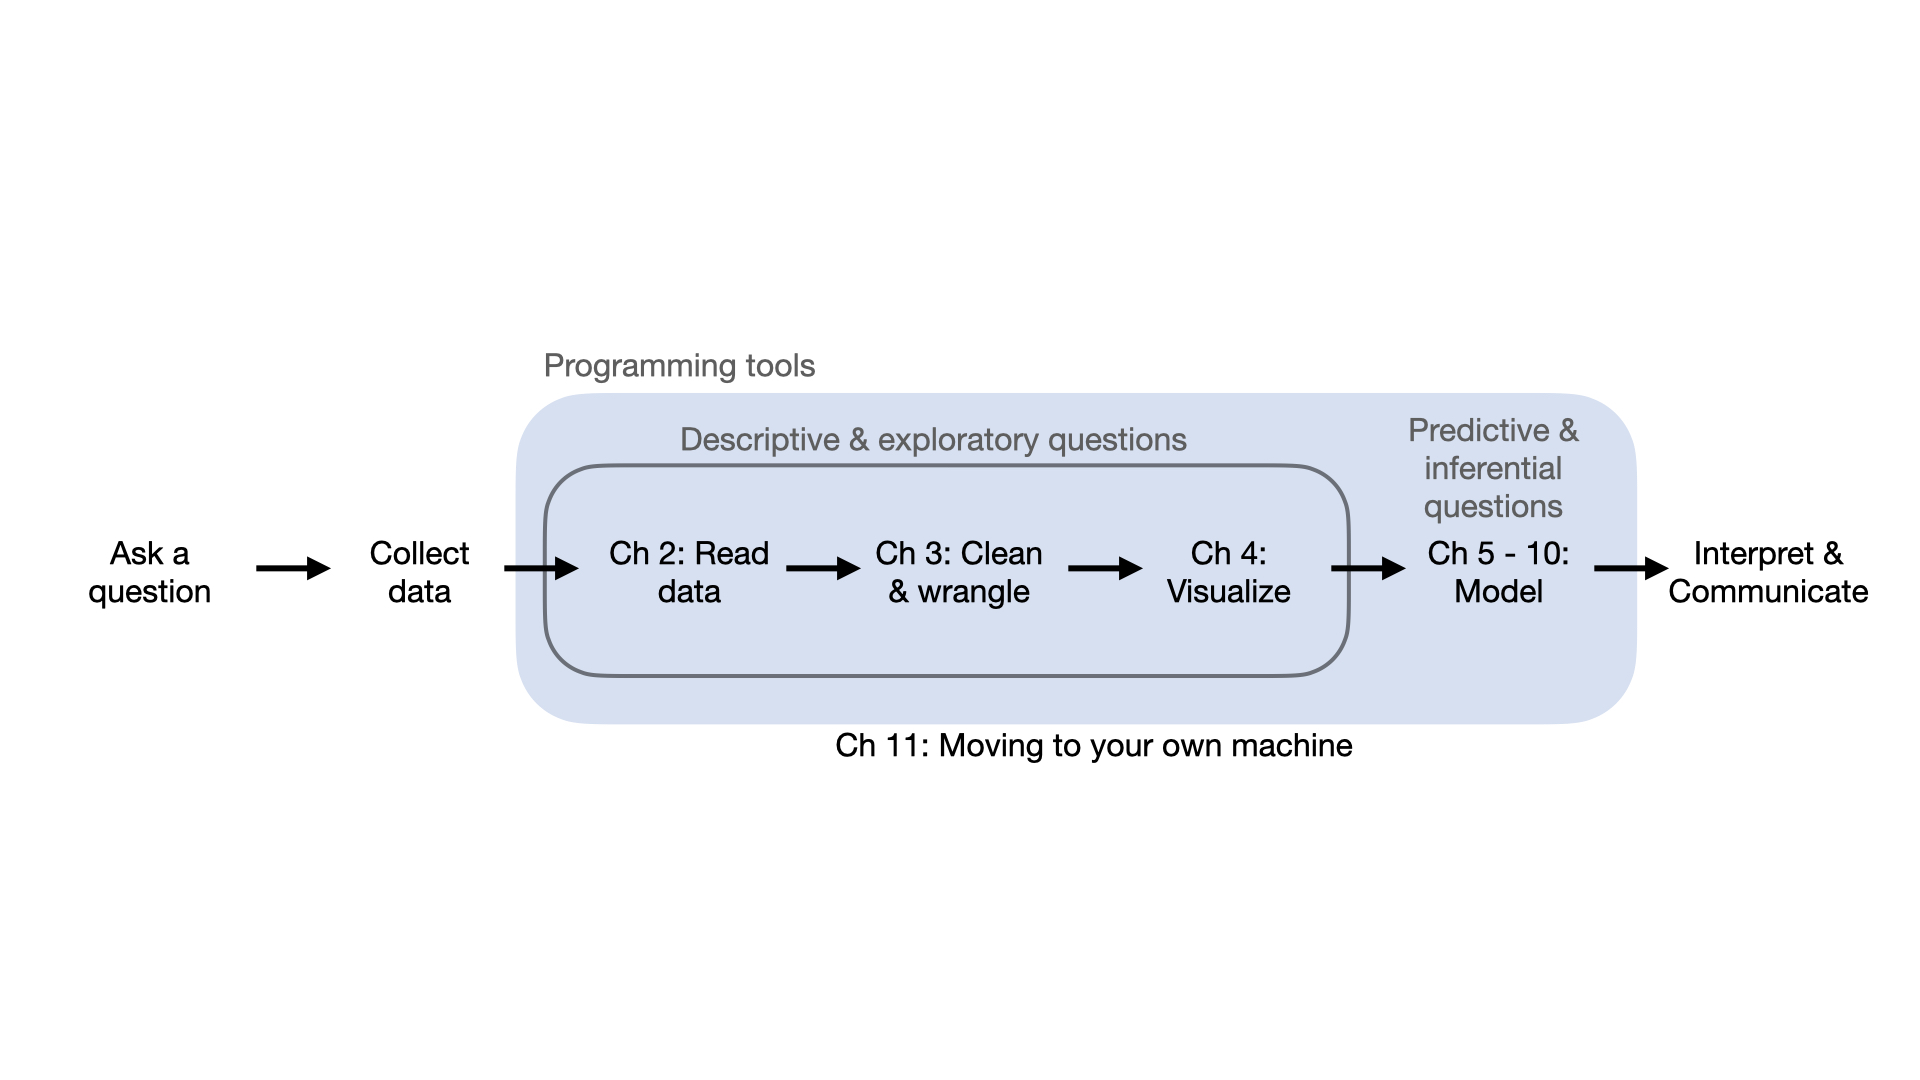
\includegraphics[width=1\linewidth]{img/chapter_overview} \caption{Where are we going?}\label{fig:img-chapter-overview}
\end{figure}

\hypertarget{intro}{%
\chapter{R and the tidyverse}\label{intro}}

\hypertarget{overview}{%
\section{Overview}\label{overview}}

This chapter provides an introduction to data science and the R programming language.
The goal here is to get your hands dirty right from the start: we will walk through an entire data analysis,
and along the way introduce different types of data analysis questions, some fundamental programming
concepts in R, and the basics of loading, cleaning, and visualizing data. In the following chapters, we will
dig into each of these steps in much more detail; but for now, let's jump in to see how much we can do
with data science!

\hypertarget{chapter-learning-objectives}{%
\section{Chapter learning objectives}\label{chapter-learning-objectives}}

By the end of the chapter, readers will be able to:

\begin{itemize}
\tightlist
\item
  identify the different types of data analysis question and categorize a question into the correct type
\item
  load the \texttt{tidyverse} package into R
\item
  read tabular data with \texttt{read\_csv}
\item
  use \texttt{?} to access help and documentation tools in R
\item
  create new variables and objects in R using the assignment symbol
\item
  create and organize subsets of tabular data using \texttt{filter}, \texttt{select}, \texttt{arrange}, and \texttt{slice}
\item
  visualize data with a \texttt{ggplot} bar plot
\end{itemize}

\hypertarget{canadian-languages-data-set}{%
\section{Canadian languages data set}\label{canadian-languages-data-set}}

In this chapter, \index{Canadian languages} we will walk through a full analysis of a data set relating to
languages spoken at home by Canadians. Many Indigenous peoples exist in Canada
with their own cultures and languages; these languages are often unique to Canada and not spoken
anywhere else in the world \citep{statcan2018mothertongue}. Sadly, colonization has
led to the loss of many of these languages. For instance, generations of
children were not allowed to speak their mother tongue (the first language an
individual learns in childhood) in Canadian residential schools. Colonizers
also renamed places they had ``discovered'' \citep{wilson2018}. Acts such as these
have significantly harmed the continuity of Indigenous languages in Canada, and
some languages are considered ``endangered'' as few people report speaking them.
To learn more, please see Canadian Geographic's article on
\href{https://www.canadiangeographic.ca/article/mapping-indigenous-languages-canada}{Mapping Indigenous languages in Canada}
\citep{walker2017}, \href{http://publications.gc.ca/site/archivee-archived.html?url=http://publications.gc.ca/collections/collection_2012/cvrc-trcc/IR4-4-2012-eng.pdf}{They Came for the Children: Canada, Aboriginal peoples, and Residential Schools} \citep{children2012}
and the Truth and Reconciliation Commission of
Canada's \href{http://trc.ca/assets/pdf/Calls_to_Action_English2.pdf}{Calls to Action} \citep{calls2015}.

The data set we will study in this chapter is taken from
\href{https://ttimbers.github.io/canlang/}{the \{canlang\} R data package} \citep{timbers2020canlang}, which has
population language data collected during the 2016 Canadian census \citep{cancensus2016}.
In this data there are 214 languages recorded, each having 6 different properties:

\begin{enumerate}
\def\labelenumi{\arabic{enumi}.}
\tightlist
\item
  \texttt{category}: Higher-level language category, describing whether the language is an Official Canadian language, an Aboriginal (i.e., Indigenous) language, or a Non-Official and Non-Aboriginal language.
\item
  \texttt{language}: The name of the language.
\item
  \texttt{mother\_tongue}: Number of Canadians who reported the language as their mother tongue. Mother tongue is generally defined as the language someone was exposed to since birth.
\item
  \texttt{most\_at\_home}: Number of Canadians who reported the language as being spoken most often at home.
\item
  \texttt{most\_at\_work}: Number of Canadians who reported the language as being used most often at work.
\item
  \texttt{lang\_known}: Number of Canadians who reported knowledge of the language.
\end{enumerate}

According to the census, more than 60 Aboriginal languages were reported
as being spoken in Canada. Suppose we want to know which are the most common;
then we might ask the following question, which we wish to answer using our data:

\emph{Which ten Aboriginal languages were most often reported in 2016 as mother
tongues in Canada, and how many people speak each of them?}

\begin{quote}
\textbf{A note about the \emph{data} in data science!}
Data science\index{data science!good practices} cannot be done without a deep understanding of the data and
problem domain. In this book, we have simplified the data sets used in our
examples to concentrate on methods and fundamental concepts. But in real
life, you cannot and should not do data science without a domain expert.
Alternatively, it is common to practice data science in your own domain of
expertise! Remember that when you work with data, it is essential to think
about \emph{how} the data were collected, which affects the conclusions you can
draw. If your data are biased, then your results will be biased!
\end{quote}

\hypertarget{asking-a-question}{%
\section{Asking a question}\label{asking-a-question}}

Every good data analysis begins with a \emph{question}---like the
above---that you aim to answer using data. As it turns out, there
are actually a number of different \emph{types} of question regarding data:
descriptive, exploratory, inferential, predictive, causal, and mechanistic,
all of which are defined in Table \ref{tab:questions-table}.
Carefully formulating a question as early as possible in your analysis---and
correctly identifying which type of question it is---will guide your overall approach to
the analysis as well as the selection of appropriate tools.\index{question!data analysis}
\index{descriptive question!definition}
\index{exploratory question!definition}
\index{predictive question!definition}
\index{inferential question!definition}
\index{causal question!definition}
\index{mechanistic question!definition}

\begin{longtable}[]{@{}
  >{\raggedright\arraybackslash}p{(\columnwidth - 4\tabcolsep) * \real{0.41}}
  >{\raggedright\arraybackslash}p{(\columnwidth - 4\tabcolsep) * \real{0.35}}
  >{\raggedright\arraybackslash}p{(\columnwidth - 4\tabcolsep) * \real{0.24}}@{}}
\caption{\label{tab:questions-table} Types of data analysis question. From \href{https://science.sciencemag.org/content/347/6228/1314}{What is the question?} \citep{leek2015question} and \href{https://leanpub.com/artofdatascience}{The Art of Data Science} \citep{peng2015art}.}\tabularnewline
\toprule
\begin{minipage}[b]{\linewidth}\raggedright
Question type
\end{minipage} & \begin{minipage}[b]{\linewidth}\raggedright
Description
\end{minipage} & \begin{minipage}[b]{\linewidth}\raggedright
Example
\end{minipage} \\
\midrule
\endfirsthead
\toprule
\begin{minipage}[b]{\linewidth}\raggedright
Question type
\end{minipage} & \begin{minipage}[b]{\linewidth}\raggedright
Description
\end{minipage} & \begin{minipage}[b]{\linewidth}\raggedright
Example
\end{minipage} \\
\midrule
\endhead
Descriptive & A question that asks about summarized characteristics of a data set without interpretation (i.e., report a fact). & How many people live in each province and territory in Canada? \\
Exploratory & A question asks if there are patterns, trends, or relationships within a single data set. Often used to propose hypotheses for future study. & Does political party voting change with indicators of wealth in a set of data collected on 2,000 people living in Canada? \\
Predictive & A question that asks about predicting measurements or labels for individuals (people or things). The focus is on what things predict some outcome, but not what causes the outcome. & What political party will someone vote for in the next Canadian election? \\
Inferential & A question that looks for patterns, trends, or relationships in a single data set \textbf{and} also asks for quantification of how applicable these findings are to the wider population. & Does political party voting change with indicators of wealth for all people living in Canada? \\
Causal & A question that asks about whether changing one factor will lead to a change in another factor, on average, in the wider population. & Does wealth lead to voting for a certain political party in Canadian elections? \\
Mechanistic & A question that asks about the underlying mechanism of the observed patterns, trends, or relationships (i.e., how does it happen?) & How does wealth lead to voting for a certain political party in Canadian elections? \\
\bottomrule
\end{longtable}

In this book, you will learn techniques to answer the
first four types of question: descriptive, exploratory, predictive, and inferential;
causal and mechanistic questions are beyond the scope of this book.
In particular, you will learn how to apply the following analysis tools:

\begin{enumerate}
\def\labelenumi{\arabic{enumi}.}
\tightlist
\item
  \textbf{Summarization:} \index{summarization!overview} computing and reporting aggregated values pertaining to a data set.
  Summarization is most often used to answer descriptive questions,
  and can occasionally help with answering exploratory questions.
  For example, you might use summarization to answer the following question:
  \emph{what is the average race time for runners in this data set?}
  Tools for summarization are covered in detail in Chapters \ref{reading}
  and \ref{wrangling}, but appear regularly throughout the text.
\item
  \textbf{Visualization:} \index{visualization!overview} plotting data graphically.
  Visualization is typically used to answer descriptive and exploratory questions,
  but plays a critical supporting role in answering all of the types of question in Table \ref{tab:questions-table}.
  For example, you might use visualization to answer the following question:
  \emph{is there any relationship between race time and age for runners in this data set?}
  This is covered in detail in Chapter \ref{viz}, but again appears regularly throughout the book.
\item
  \textbf{Classification:} \index{classification!overview} predicting a class or category for a new observation.
  Classification is used to answer predictive questions.
  For example, you might use classification to answer the following question:
  \emph{given measurements of a tumour's average cell area and perimeter, is the tumour benign or malignant?}
  Classification is covered in Chapters \ref{classification} and \ref{classification2}.
\item
  \textbf{Regression:} \index{regression!overview} predicting a quantitative value for a new observation.
  Regression is also used to answer predictive questions.
  For example, you might use regression to answer the following question:
  \emph{what will be the race time for a 20-year-old runner who weighs 50kg?}
  Regression is covered in Chapters \ref{regression1} and \ref{regression2}.
\item
  \textbf{Clustering:} \index{clustering!overview} finding previously unknown/unlabelled subgroups in a
  dataset. Clustering is often used to answer exploratory questions.
  For example, you might use clustering to answer the following question:
  \emph{what products are commonly bought together on Amazon?}
  Clustering is covered in Chapter \ref{clustering}.
\item
  \textbf{Estimation:} \index{estimation!overview} taking measurements for small number of items from a large group
  and making a good guess for the average or proportion for the large group. Estimation
  is used to answer inferential questions.
  For example, you might use estimation to answer the following question:
  \emph{Given a survey of cellphone ownership of 100 Canadians, what proportion
  of the entire Canadian population own Android phones?}
  Estimation is covered in Chapter \ref{inference}.
\end{enumerate}

Referring to Table \ref{tab:questions-table}, our question about
Aboriginal languages is an example of a \emph{descriptive question}: we are
summarizing the characteristics of a data set without further interpretation.
And referring to the list above, it looks like we should use visualization
and perhaps some summarization to answer the question. So in the remainder
of this chapter, we will work towards making a visualization that shows
us the ten most common Aboriginal languages in Canada and their associated counts,
according to the 2016 census.

\hypertarget{loading-a-tabular-data-set}{%
\section{Loading a tabular data set}\label{loading-a-tabular-data-set}}

A data set is, at its core essence, a structured collection of numbers and characters.
Aside from that, there are really no strict rules; data sets can come in
many different forms! Perhaps the most common form of data set that you will
find in the wild, however, is \emph{tabular data}\index{tabular data}. Think spreadsheets in Microsoft Excel: tabular data are
rectangular-shaped and spreadsheet-like, as shown in Figure
\ref{fig:img-spreadsheet-vs-dataframe}. In this book, we will focus primarily on tabular data.

Since we are using R for data analysis in this book, the first step for us is to
load the data into R. When we load tabular data into
R, it is represented as a \emph{data frame} object\index{data frame!overview}. Figure
\ref{fig:img-spreadsheet-vs-dataframe} shows that an R data frame is very similar
to a spreadsheet. We refer to the rows as \index{observation} \textbf{observations}; these are the things that we
collect the data on, e.g., voters, cities, etc. We refer to the columns as \index{variable}
\textbf{variables}; these are the characteristics of those observations, e.g., voters' political
affiliations, cities' populations, etc.

\begin{figure}
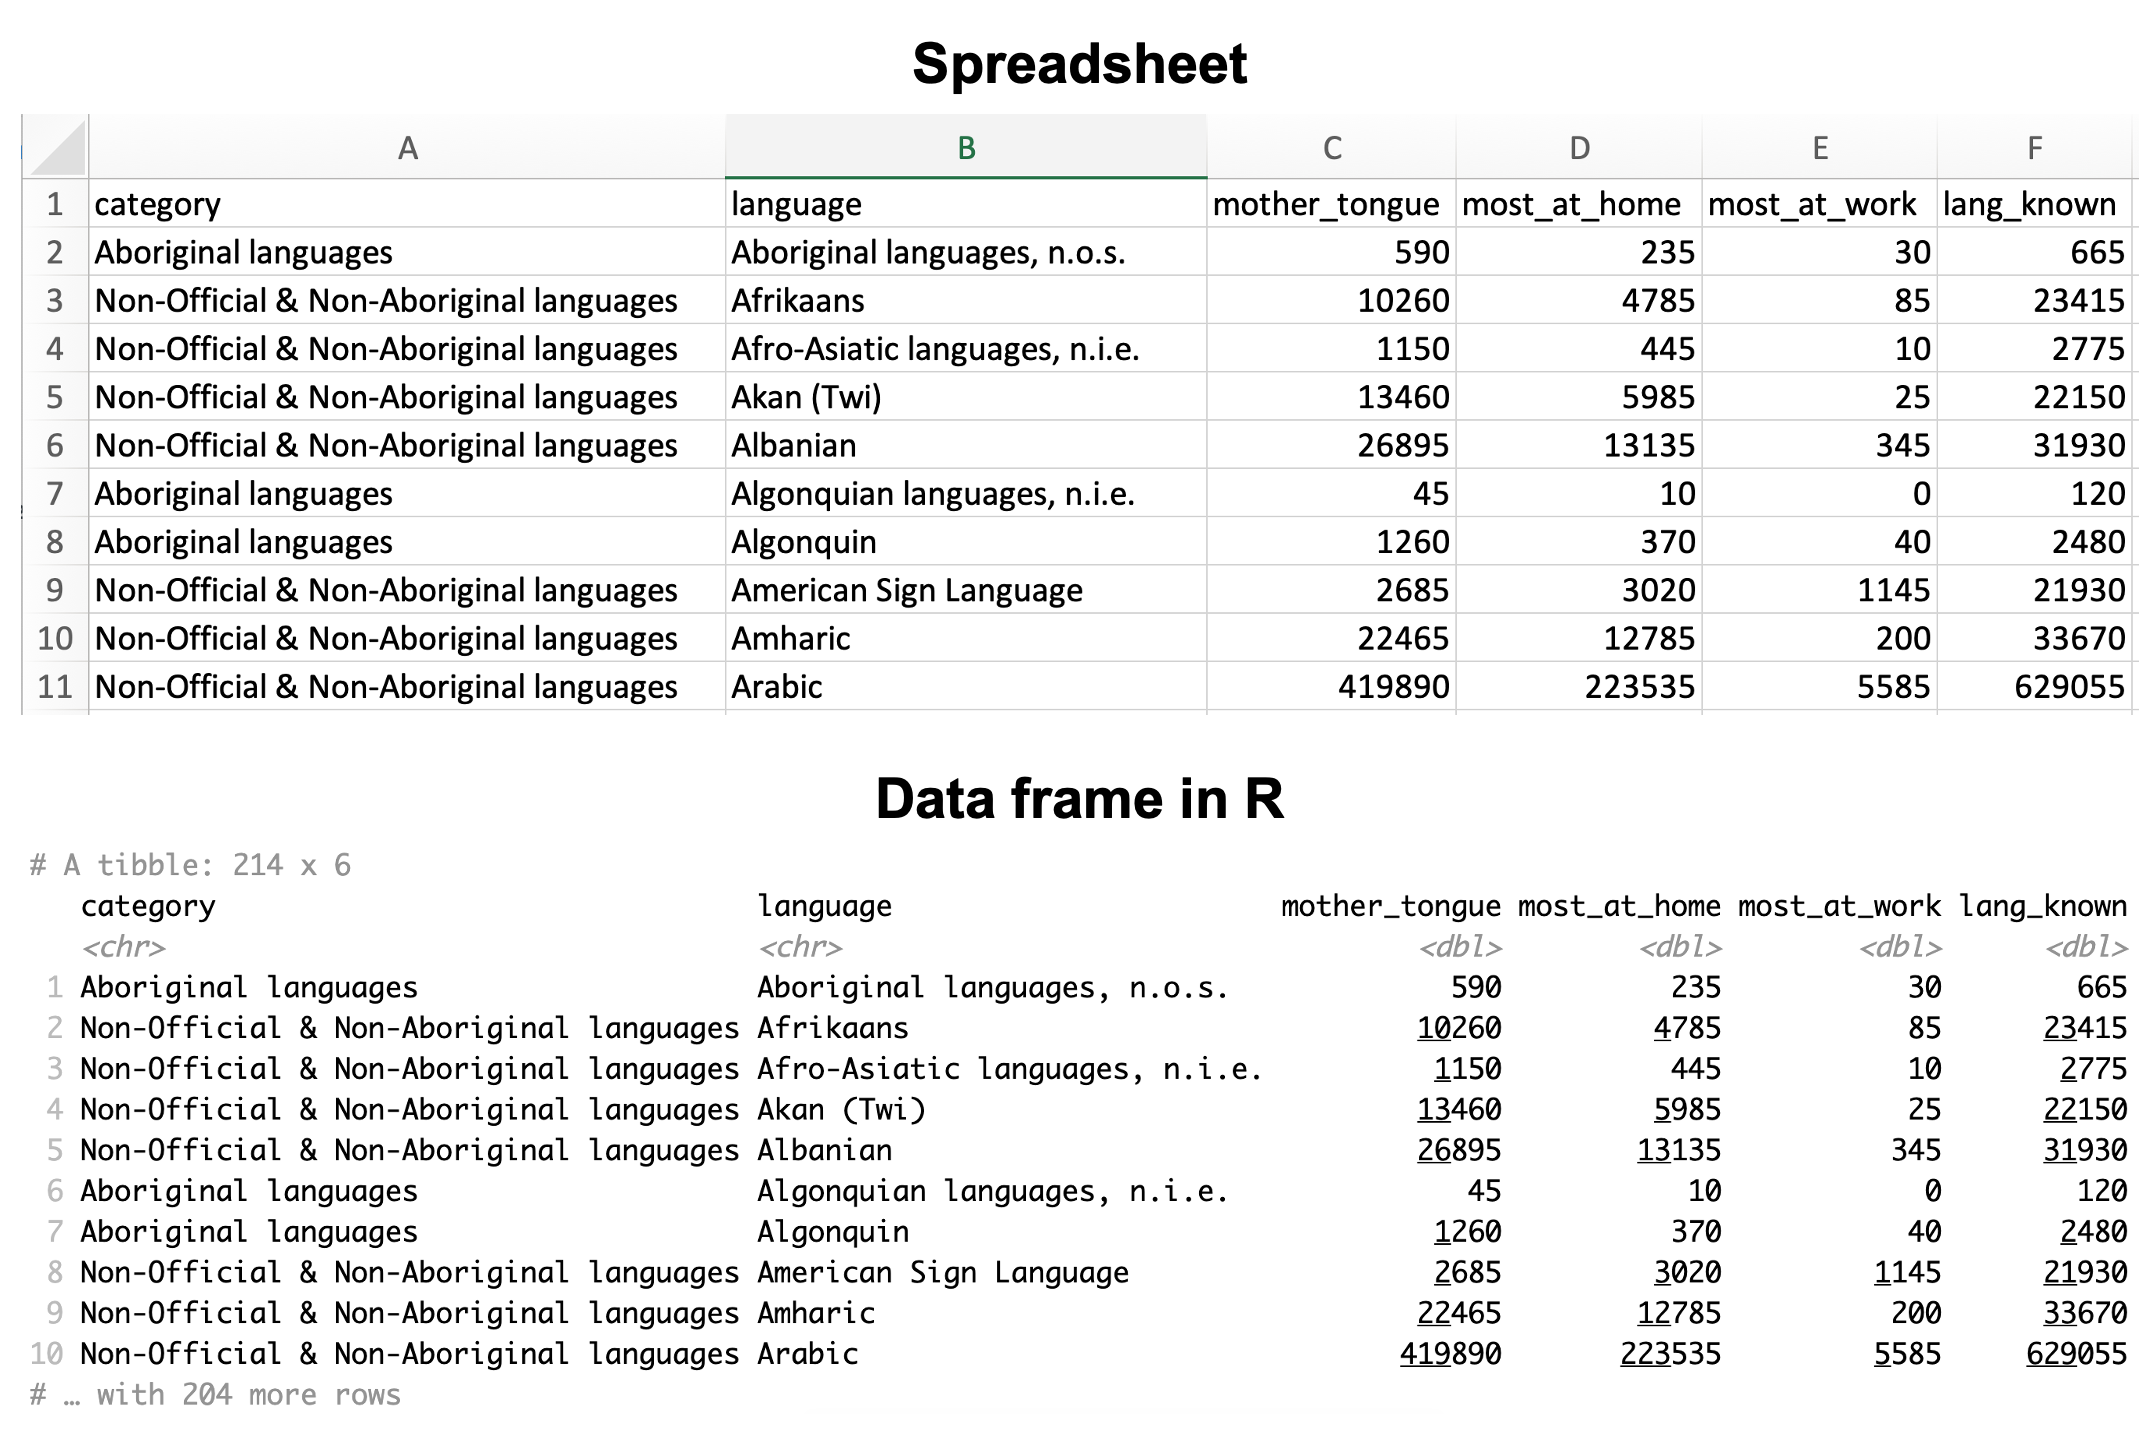
\includegraphics[width=850pt]{img/spreadsheet_vs_dataframe} \caption{A spreadsheet versus a data frame in R}\label{fig:img-spreadsheet-vs-dataframe}
\end{figure}

The first kind of data file that we will learn how to load into R as a data
frame is the \emph{comma-separated values} format (\texttt{.csv} for short)\index{comma-separated values|see{csv}}\index{csv}. These files
have names ending in \texttt{.csv}, and can be opened and saved using common
spreadsheet programs like Microsoft Excel and Google Sheets. For example, the
\texttt{.csv} file named \texttt{can\_lang.csv}
\href{https://raw.githubusercontent.com/UBC-DSCI/introduction-to-datascience/master/data/can_lang.csv}{is included with the code for this book}.
If we were to open this data in a plain text editor (a program like Notepad that just shows
text with no formatting), we would see each row on its own line, and each entry in the table separated by a comma:

\begin{verbatim}
category,language,mother_tongue,most_at_home,most_at_work,lang_known
Aboriginal languages,"Aboriginal languages, n.o.s.",590,235,30,665
Non-Official & Non-Aboriginal languages,Afrikaans,10260,4785,85,23415
Non-Official & Non-Aboriginal languages,"Afro-Asiatic languages, n.i.e.",1150,445,10,2775
Non-Official & Non-Aboriginal languages,Akan (Twi),13460,5985,25,22150
Non-Official & Non-Aboriginal languages,Albanian,26895,13135,345,31930
Aboriginal languages,"Algonquian languages, n.i.e.",45,10,0,120
Aboriginal languages,Algonquin,1260,370,40,2480
Non-Official & Non-Aboriginal languages,American Sign Language,2685,3020,1145,21930
Non-Official & Non-Aboriginal languages,Amharic,22465,12785,200,33670
\end{verbatim}

To load this data into R so that we can do things with it (e.g, perform
analyses or create data visualizations), we will need to use a \emph{function.} \index{function} A
function is a special word in R that takes instructions (we call these
\emph{arguments}) \index{argument} and does something. The function we will use to load a \texttt{.csv} file
into R is called \texttt{read\_csv}. \index{read function!read\_csv} In its most basic
use-case, \texttt{read\_csv} expects that the data file:

\begin{itemize}
\tightlist
\item
  has column names (or \emph{headers}),
\item
  uses a comma (\texttt{,}) to separate the columns, and
\item
  does not have row names.
\end{itemize}

Below you'll see the code used to load the data into R using the \texttt{read\_csv}
function. Note that the \texttt{read\_csv} function is not included in the base
installation of R, meaning that it is not one of the primary functions ready to
use when you install R. Therefore, you need to load it from somewhere else
before you can use it. The place from which we will load it is called an R \emph{package}.
An R package \index{package} is a collection of functions that can be used in addition to the
built-in R package functions once loaded. The \texttt{read\_csv} function, in
particular, can be made accessible by loading the \texttt{tidyverse} package \citep{wickham2019tidverse}
using the \texttt{library} function. \index{library} The \texttt{tidyverse} \index{tidyverse} package contains many
functions that we will use throughout this book to load, clean, wrangle,
and visualize data.

\begin{Shaded}
\begin{Highlighting}[]
\FunctionTok{library}\NormalTok{(tidyverse)}
\end{Highlighting}
\end{Shaded}

\begin{verbatim}
## -- Attaching packages --------------------------------------------------------------------------------- tidyverse 1.3.1 --
\end{verbatim}

\begin{verbatim}
## v ggplot2 3.3.5     v purrr   0.3.4
## v tibble  3.1.2     v dplyr   1.0.6
## v tidyr   1.1.3     v stringr 1.4.0
## v readr   2.0.1
\end{verbatim}

\begin{verbatim}
## -- Conflicts ------------------------------------------------------------------------------------ tidyverse_conflicts() --
## x dplyr::filter() masks stats::filter()
## x dplyr::lag()    masks stats::lag()
\end{verbatim}

\begin{quote}
\textbf{In case you want to know more (optional):} Notice that we got some extra
output from R saying \texttt{Attaching\ packages} and \texttt{Conflicts} below our code
line. These are examples of \emph{messages} in R, which give the user more
information that might be handy to know. The \texttt{Attaching\ packages} message is
natural when loading \texttt{tidyverse}, since \texttt{tidyverse} actually automatically
causes other packages to be imported too, such as \texttt{dplyr}. In the future
when we load \texttt{tidyverse} in this book we will silence these messages to help
with readability of the book. The \texttt{Conflicts} message is also totally normal
in this circumstance. This message tells you if functions from different
packages share the same name, which is confusing to R. For example, in this
case, the \texttt{dplyr} package and the \texttt{stats} package both provide a function
called \texttt{filter}. The message above (\texttt{dplyr::filter()\ masks\ stats::filter()})
is R telling you that it is going to default to the \texttt{dplyr} package version
of this function. So if you use the \texttt{filter} function, you will be using the
\texttt{dplyr} version. In order to use the \texttt{stats} version, you need to use its
full name \texttt{stats::filter}. Messages are not errors, so generally you don't
need to take action when you see a message; but you should always read the message
and critically think about what it means and whether you need to do anything
about it.
\end{quote}

After loading the \texttt{tidyverse} package, we can call the \texttt{read\_csv} function and
pass it a single argument: the name of the file, \texttt{"can\_lang.csv"}. We have to
put quotes around file names and other letters and words that we use in our
code to distinguish it from the special words (like functions!) that make up the R programming
language. The file's name is the only argument we need to provide because our
file satisfies everything else that the \texttt{read\_csv} function expects in the default
use-case. Figure \ref{fig:img-read-csv} describes how we use the \texttt{read\_csv}
to read data into R.

\begin{figure}
\centering
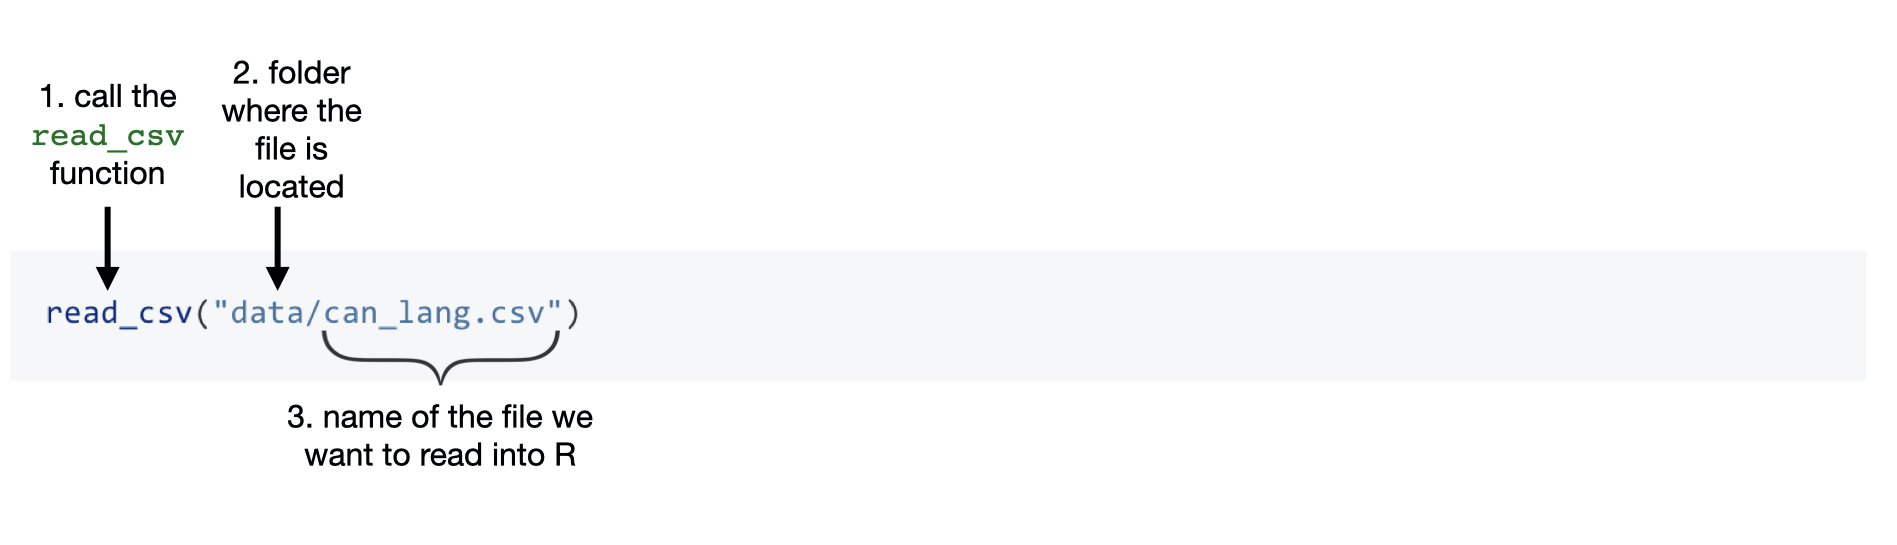
\includegraphics{img/read_csv_function.jpeg}
\caption{\label{fig:img-read-csv}Syntax for the \texttt{read\_csv} function.}
\end{figure}

\begin{Shaded}
\begin{Highlighting}[]
\FunctionTok{read\_csv}\NormalTok{(}\StringTok{"data/can\_lang.csv"}\NormalTok{)}
\end{Highlighting}
\end{Shaded}

\begin{verbatim}
## # A tibble: 214 x 6
##    category       language    mother_tongue most_at_home most_at_work lang_known
##    <chr>          <chr>               <dbl>        <dbl>        <dbl>      <dbl>
##  1 Aboriginal la~ Aboriginal~           590          235           30        665
##  2 Non-Official ~ Afrikaans           10260         4785           85      23415
##  3 Non-Official ~ Afro-Asiat~          1150          445           10       2775
##  4 Non-Official ~ Akan (Twi)          13460         5985           25      22150
##  5 Non-Official ~ Albanian            26895        13135          345      31930
##  6 Aboriginal la~ Algonquian~            45           10            0        120
##  7 Aboriginal la~ Algonquin            1260          370           40       2480
##  8 Non-Official ~ American S~          2685         3020         1145      21930
##  9 Non-Official ~ Amharic             22465        12785          200      33670
## 10 Non-Official ~ Arabic             419890       223535         5585     629055
## # ... with 204 more rows
\end{verbatim}

\begin{quote}
\textbf{In case you want to know more (optional):} There is another function
that also loads csv files named \texttt{read.csv}. We will \emph{always} use
\texttt{read\_csv} in this book, as it is designed to play nicely with all of the
other \texttt{tidyverse} functions, which we will use extensively. Be
careful not to accidentally use \texttt{read.csv}, as it can cause some tricky
errors to occur in your code that are hard to track down!
\end{quote}

\hypertarget{naming-things-in-r}{%
\section{Naming things in R}\label{naming-things-in-r}}

When we loaded the 2016 Canadian census language data
using \texttt{read\_csv}, we did not give this data frame a name.
Therefore the data was just printed on the screen,
and we cannot do anything else with it. That isn't very useful.
What would be more useful would be to give a name
to the data frame that \texttt{read\_csv} outputs,
so that we can refer to it later for analysis and visualization.

The way to assign a name to a value in R is via the \emph{assignment symbol} \texttt{\textless{}-}.
\index{assignsymb@\texttt{<-}|see{assignment symbol}}\index{assignment symbol}
On the left side of the assignment symbol you put the name that you want
to use, and on the right side of the assignment symbol
you put the value that you want the name to refer to.
Names can be used to refer to almost anything in R, such as numbers,
words (also known as \emph{strings} of characters), and data frames!
Below, we set \texttt{my\_number} to \texttt{3} (the result of \texttt{1+2})
and we set \texttt{name} to the string \texttt{"Alice"}. \index{string}

\begin{Shaded}
\begin{Highlighting}[]
\NormalTok{my\_number }\OtherTok{\textless{}{-}} \DecValTok{1} \SpecialCharTok{+} \DecValTok{2}
\NormalTok{name }\OtherTok{\textless{}{-}} \StringTok{"Alice"}
\end{Highlighting}
\end{Shaded}

Note that when
we name something in R using the assignment symbol, \texttt{\textless{}-},
we do not need to surround the name we are creating with quotes. This is
because we are formally telling R that this special word denotes
the value of whatever is on the right hand side.
Only characters and words that act as \emph{values} on the right hand side of the assignment
symbol---e.g., the file name \texttt{"data/can\_lang.csv"} that we specified before, or \texttt{"Alice"} above------need
to be surrounded by quotes.

After making the assignment, we can use the special name words we have created in
place of their values. For example, if we want to do something with the value \texttt{3} later on,
we can just use \texttt{my\_number} instead. Let's try adding 2 to \texttt{my\_number}; you will see that
R just interprets this as adding 2 and 3:

\begin{Shaded}
\begin{Highlighting}[]
\NormalTok{my\_number }\SpecialCharTok{+} \DecValTok{2}
\end{Highlighting}
\end{Shaded}

\begin{verbatim}
## [1] 5
\end{verbatim}

Object names \index{object} can consist of letters, numbers, periods \texttt{.} and underscores \texttt{\_}.
Other symbols won't work since they have their own meanings in R. For example,
\texttt{+} is the addition symbol; if we try to assign a name with
the \texttt{+} symbol, R will complain and we will get an error!

\begin{Shaded}
\begin{Highlighting}[]
\NormalTok{na}\SpecialCharTok{+}\NormalTok{me }\OtherTok{\textless{}{-}} \DecValTok{1}
\end{Highlighting}
\end{Shaded}

\begin{verbatim}
Error: unexpected assignment in "na+me <-"
\end{verbatim}

There are certain conventions for naming objects in R. When naming \index{object!naming convention} an object we
suggest using only lower case letters, numbers and underscores \texttt{\_} to separate
the words in a name. R is case sensitive, which means that \texttt{Letter} and
\texttt{letter} would be two different objects in R. You should also try to give your
objects meaningful names. For instance, you \emph{can} name a data frame \texttt{x}.
However, using more meaningful terms, such as \texttt{language\_data}, will help you
remember what each name in your code represents. We recommend following the
Tidyverse naming conventions outlined in the \href{https://principles.tidyverse.org/names-attribute.html\#universal-names}{Tidyverse Style
Guide}
\citep{tidyversestyleguide}. Let's now use the assignment symbol to give the name
\texttt{can\_lang} to the 2016 Canadian census language data frame that we get from
\texttt{read\_csv}.

\begin{Shaded}
\begin{Highlighting}[]
\NormalTok{can\_lang }\OtherTok{\textless{}{-}} \FunctionTok{read\_csv}\NormalTok{(}\StringTok{"data/can\_lang.csv"}\NormalTok{)}
\end{Highlighting}
\end{Shaded}

Wait a minute, nothing happened this time! Where's our data?
Actually, something did happen: the data was loaded in
and now has the name \texttt{can\_lang} associated with it.
And we can use that name to access the data frame and do things with it.
For example, we can type the name of the data frame to print the first few rows
on the screen. You will also see at the top that the number of observations (i.e., rows) and
variables (i.e., columns) are printed. Printing the first few rows of a data frame
like this is a handy way to get a quick sense for what is contained in a data frame.

\begin{Shaded}
\begin{Highlighting}[]
\NormalTok{can\_lang}
\end{Highlighting}
\end{Shaded}

\begin{verbatim}
## # A tibble: 214 x 6
##    category       language    mother_tongue most_at_home most_at_work lang_known
##    <chr>          <chr>               <dbl>        <dbl>        <dbl>      <dbl>
##  1 Aboriginal la~ Aboriginal~           590          235           30        665
##  2 Non-Official ~ Afrikaans           10260         4785           85      23415
##  3 Non-Official ~ Afro-Asiat~          1150          445           10       2775
##  4 Non-Official ~ Akan (Twi)          13460         5985           25      22150
##  5 Non-Official ~ Albanian            26895        13135          345      31930
##  6 Aboriginal la~ Algonquian~            45           10            0        120
##  7 Aboriginal la~ Algonquin            1260          370           40       2480
##  8 Non-Official ~ American S~          2685         3020         1145      21930
##  9 Non-Official ~ Amharic             22465        12785          200      33670
## 10 Non-Official ~ Arabic             419890       223535         5585     629055
## # ... with 204 more rows
\end{verbatim}

\hypertarget{creating-subsets-of-data-frames-with-filter-select}{%
\section{\texorpdfstring{Creating subsets of data frames with \texttt{filter} \& \texttt{select}}{Creating subsets of data frames with filter \& select}}\label{creating-subsets-of-data-frames-with-filter-select}}

Now that we've loaded our data into R, we can start wrangling the data to
find the ten Aboriginal languages that were most often reported
in 2016 as mother tongues in Canada. In particular, we will construct
a table with the ten Aboriginal languages that have the largest
counts in the \texttt{mother\_tongue} column.
The \texttt{filter} and \texttt{select} functions from the \texttt{tidyverse} package will help us
here. The \texttt{filter} \index{filter} function allows you to obtain a subset of the
rows with specific values, while the \texttt{select} \index{select} function allows you
to obtain a subset of the columns. Therefore, we can \texttt{filter} the rows to extract the
Aboriginal languages in the data set, and then use \texttt{select} to obtain only the
columns we want to include in our table.

\hypertarget{using-filter-to-extract-rows}{%
\subsection{\texorpdfstring{Using \texttt{filter} to extract rows}{Using filter to extract rows}}\label{using-filter-to-extract-rows}}

Looking at the \texttt{can\_lang} data above, we see the column \texttt{category} contains different
high-level categories of languages, which include ``Aboriginal languages'',
``Non-Official \& Non-Aboriginal languages'' and ``Official languages''. To answer
our question we want to filter our data set so we restrict our attention
to only those languages in the ``Aboriginal languages'' category.

We can use the \texttt{filter} \index{filter} function to obtain the subset of rows with desired
values from a data frame. Figure \ref{fig:img-filter} outlines what arguments we need to specify to use \texttt{filter}. The first argument to \texttt{filter} is the name of the data frame
object, \texttt{can\_lang}. The second argument is a \emph{logical statement} \index{logical statement} to use when
filtering the rows. A logical statement evaluates to either \texttt{TRUE} or \texttt{FALSE};
\texttt{filter} keeps only those rows for which the logical statement evaluates to \texttt{TRUE}.
For example, in our analysis, we are interested in keeping only languages in the
``Aboriginal languages'' higher-level category. We can use
the \emph{equivalency operator} \texttt{==} \index{logical statement!equivalency operator} to compare the values
of the \texttt{category} column with the value \texttt{"Aboriginal\ languages"}; you will learn about
many other kinds of logical statement in Chapter \ref{wrangling}. Similar to
when we loaded the data file and put quotes around the filename, here we need
to put quotes around \texttt{"Aboriginal\ languages"}. Using quotes tells R that this
is a string \emph{value} \index{string} and not one of the special words that make up R
programming language, nor one of the names we have given to data frames in the
code we have already written.

\begin{figure}
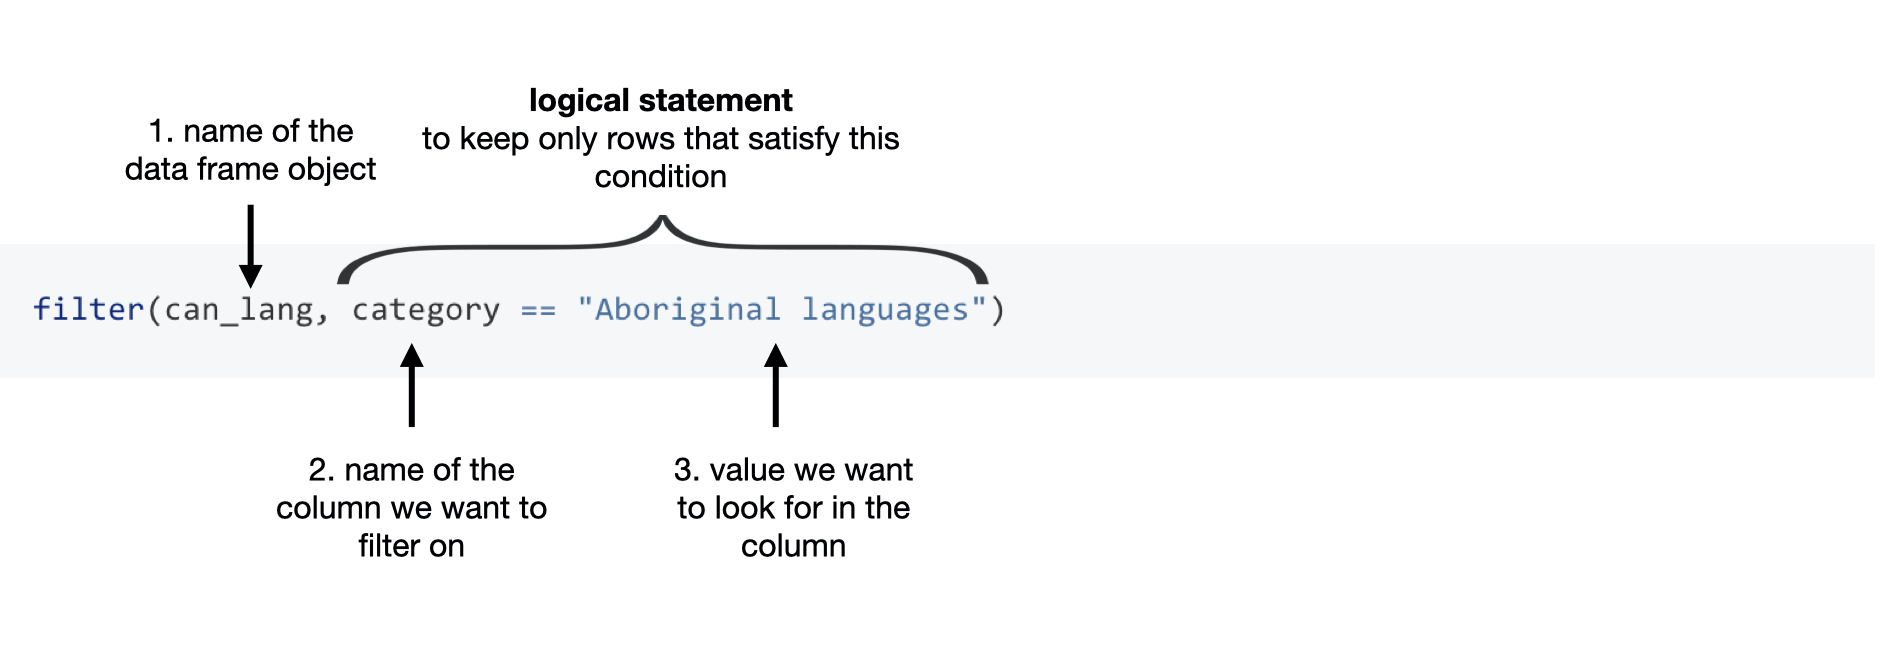
\includegraphics[width=1\linewidth]{img/filter_function} \caption{Syntax for the filter function}\label{fig:img-filter}
\end{figure}

With these arguments, \texttt{filter} returns a data frame that has all the columns of
the input data frame, but only those rows we asked for in our logical filter
statement.

\begin{Shaded}
\begin{Highlighting}[]
\NormalTok{aboriginal\_lang }\OtherTok{\textless{}{-}} \FunctionTok{filter}\NormalTok{(can\_lang, category }\SpecialCharTok{==} \StringTok{"Aboriginal languages"}\NormalTok{)}
\NormalTok{aboriginal\_lang}
\end{Highlighting}
\end{Shaded}

\begin{verbatim}
## # A tibble: 67 x 6
##    category     language      mother_tongue most_at_home most_at_work lang_known
##    <chr>        <chr>                 <dbl>        <dbl>        <dbl>      <dbl>
##  1 Aboriginal ~ Aboriginal l~           590          235           30        665
##  2 Aboriginal ~ Algonquian l~            45           10            0        120
##  3 Aboriginal ~ Algonquin              1260          370           40       2480
##  4 Aboriginal ~ Athabaskan l~            50           10            0         85
##  5 Aboriginal ~ Atikamekw              6150         5465         1100       6645
##  6 Aboriginal ~ Babine (Wets~           110           20           10        210
##  7 Aboriginal ~ Beaver                  190           50            0        340
##  8 Aboriginal ~ Blackfoot              2815         1110           85       5645
##  9 Aboriginal ~ Carrier                1025          250           15       2100
## 10 Aboriginal ~ Cayuga                   45           10           10        125
## # ... with 57 more rows
\end{verbatim}

It's good practice to check the output after using a
function in R. We can see the original \texttt{can\_lang} data set contained 214 rows
with multiple kinds of \texttt{category}. The data frame
\texttt{aboriginal\_lang} contains only 67 rows, and looks like it only contains languages in
the ``Aboriginal languages'' in the \texttt{category} column. So it looks like the function
gave us the result we wanted!

\hypertarget{using-select-to-extract-columns}{%
\subsection{\texorpdfstring{Using \texttt{select} to extract columns}{Using select to extract columns}}\label{using-select-to-extract-columns}}

Now let's use \texttt{select} \index{select} to extract the \texttt{language} and \texttt{mother\_tongue} columns
from this data frame. Figure \ref{fig:img-select} shows us the syntax for the \texttt{select} function. To extract these columns, we need to provide the \texttt{select}
function with three arguments. The first argument is the name of the data frame
object, which in this example is \texttt{aboriginal\_lang}. The second and third
arguments are the column names that we want to select: \texttt{language} and
\texttt{mother\_tongue}. After passing these three arguments, the \texttt{select} function
returns two columns (the \texttt{language} and \texttt{mother\_tongue} columns that we asked
for) as a data frame. This code is also a great example of why being
able to name things in R is useful: you can see that we are using the
result of our earlier \texttt{filter} step (which we named \texttt{aboriginal\_lang}) here
in the next step of the analysis!

\begin{figure}
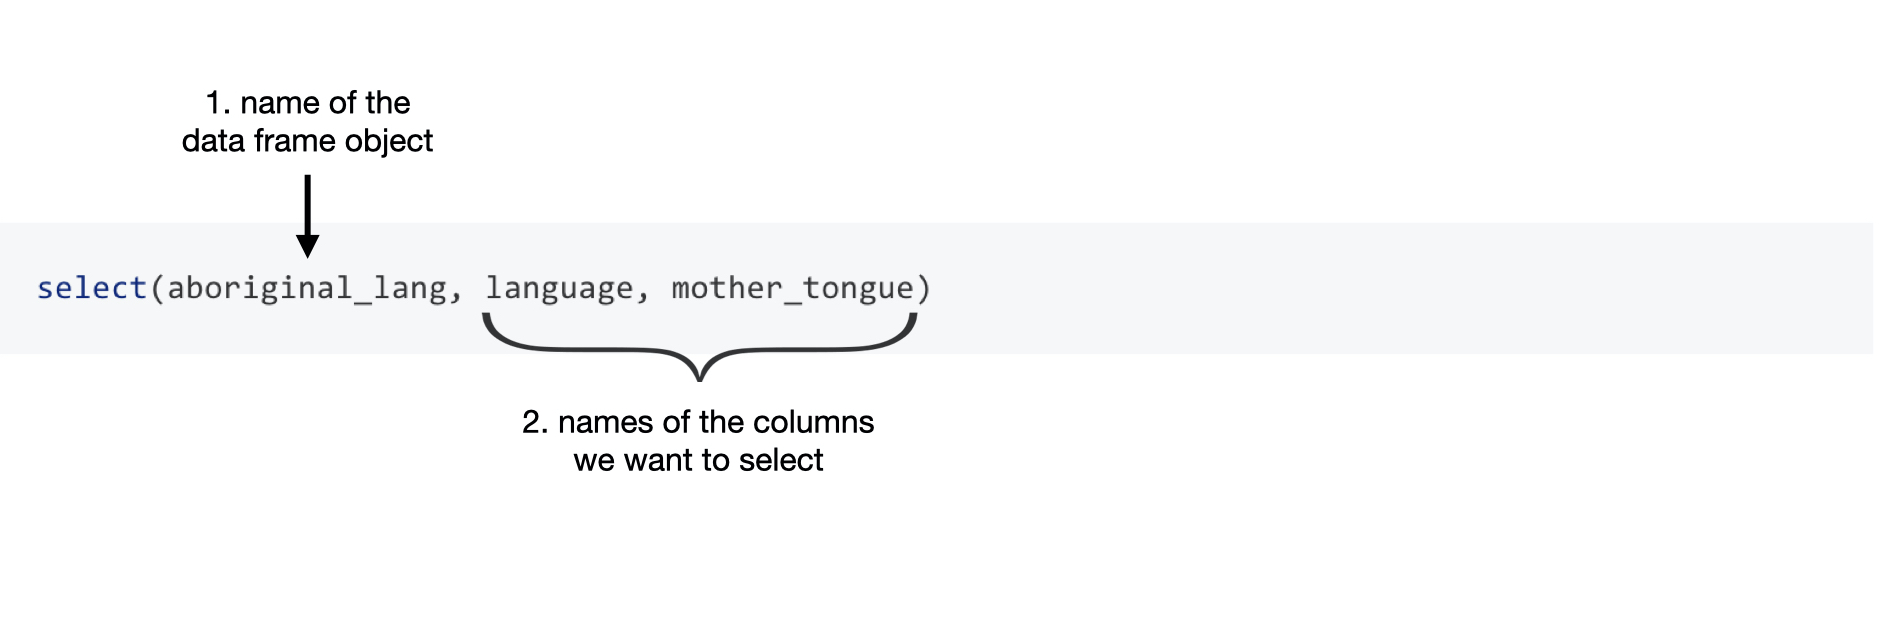
\includegraphics[width=1100pt]{img/select_function} \caption{Syntax for the select function}\label{fig:img-select}
\end{figure}

\begin{Shaded}
\begin{Highlighting}[]
\NormalTok{selected\_lang }\OtherTok{\textless{}{-}} \FunctionTok{select}\NormalTok{(aboriginal\_lang, language, mother\_tongue)}
\NormalTok{selected\_lang}
\end{Highlighting}
\end{Shaded}

\begin{verbatim}
## # A tibble: 67 x 2
##    language                     mother_tongue
##    <chr>                                <dbl>
##  1 Aboriginal languages, n.o.s.           590
##  2 Algonquian languages, n.i.e.            45
##  3 Algonquin                             1260
##  4 Athabaskan languages, n.i.e.            50
##  5 Atikamekw                             6150
##  6 Babine (Wetsuwet'en)                   110
##  7 Beaver                                 190
##  8 Blackfoot                             2815
##  9 Carrier                               1025
## 10 Cayuga                                  45
## # ... with 57 more rows
\end{verbatim}

\hypertarget{using-arrange-to-order-and-slice-to-select-rows-by-index-number}{%
\subsection{\texorpdfstring{Using \texttt{arrange} to order and \texttt{slice} to select rows by index number}{Using arrange to order and slice to select rows by index number}}\label{using-arrange-to-order-and-slice-to-select-rows-by-index-number}}

We have used \texttt{filter} and \texttt{select} to obtain a table with only the Aboriginal
languages in the data set and their associated counts. However, we want to know
the \textbf{ten} languages that are spoken most often. As a next step, we could
order the \texttt{mother\_tongue} column from greatest to least and then extract only
the top ten rows. This is where the \texttt{arrange} and \texttt{slice} functions come to the
rescue! \index{arrange}\index{slice}

The \texttt{arrange} function allows us to order the rows of a data frame by the
values of a particular column. Figure \ref{fig:img-arrange} details what arguments we need to specify to
use the \texttt{arrange} function. We need to pass the data frame as the first
argument to this function, and the variable to order by as the second argument.
Since we want to choose the ten Aboriginal languages most often reported as a mother tongue
language, we will use the \texttt{arrange} function to order the rows in our
\texttt{selected\_lang} data frame by the \texttt{mother\_tongue} column. We want to
arrange the rows in descending order (from largest to smallest),
so we pass the column to the \texttt{desc} function before using it as an argument.

\begin{figure}
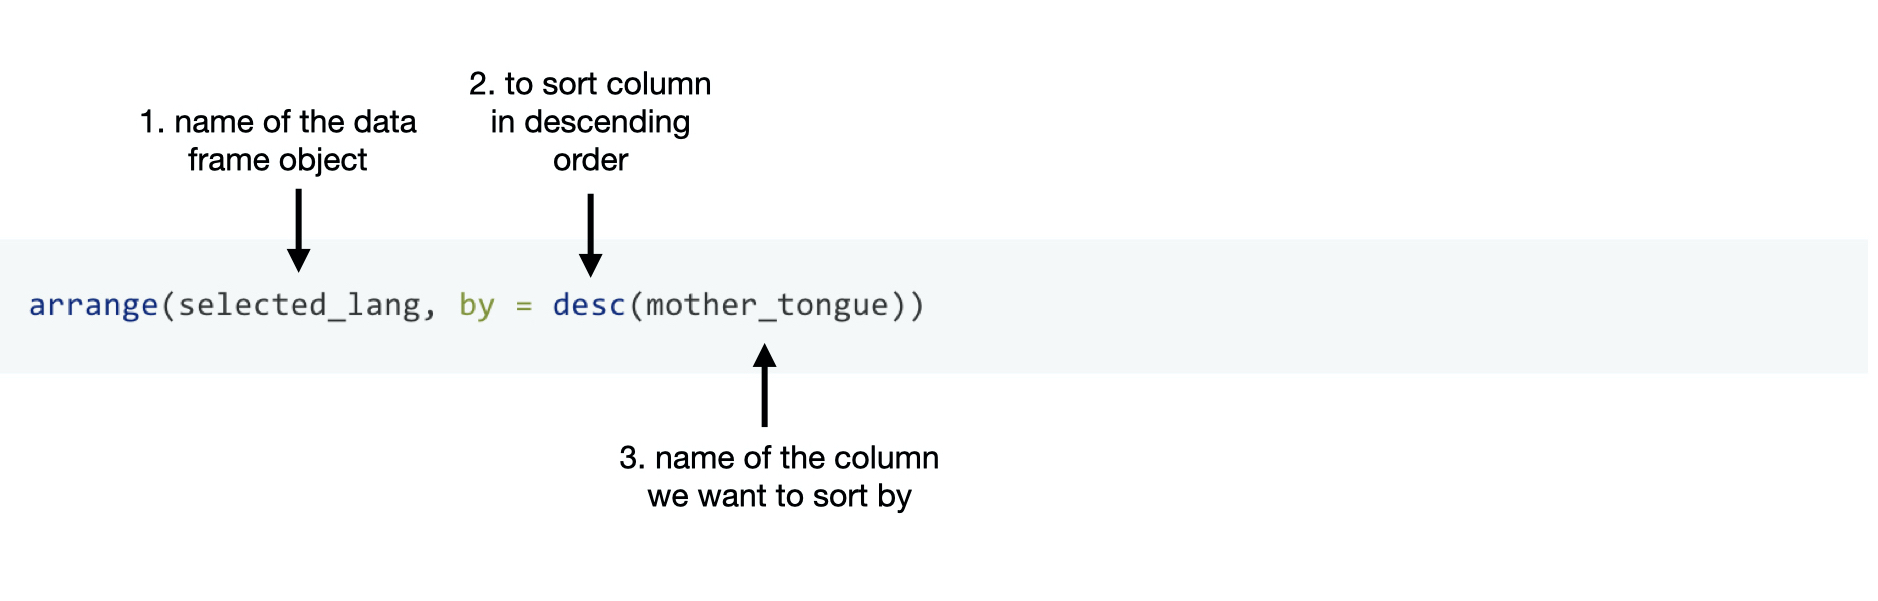
\includegraphics[width=1000pt]{img/arrange_function} \caption{Syntax for the arrange function}\label{fig:img-arrange}
\end{figure}

\begin{Shaded}
\begin{Highlighting}[]
\NormalTok{arranged\_lang }\OtherTok{\textless{}{-}} \FunctionTok{arrange}\NormalTok{(selected\_lang, }\AttributeTok{by =} \FunctionTok{desc}\NormalTok{(mother\_tongue))}
\NormalTok{arranged\_lang}
\end{Highlighting}
\end{Shaded}

\begin{verbatim}
## # A tibble: 67 x 2
##    language          mother_tongue
##    <chr>                     <dbl>
##  1 Cree, n.o.s.              64050
##  2 Inuktitut                 35210
##  3 Ojibway                   17885
##  4 Oji-Cree                  12855
##  5 Dene                      10700
##  6 Montagnais (Innu)         10235
##  7 Mi'kmaq                    6690
##  8 Atikamekw                  6150
##  9 Plains Cree                3065
## 10 Stoney                     3025
## # ... with 57 more rows
\end{verbatim}

Next we will use the \texttt{slice} function, which selects rows according to their
row number. Since we want to choose the most common ten languages, we will indicate we want the
rows 1 to 10 using the argument \texttt{1:10}.

\begin{Shaded}
\begin{Highlighting}[]
\NormalTok{ten\_lang }\OtherTok{\textless{}{-}} \FunctionTok{slice}\NormalTok{(arranged\_lang, }\DecValTok{1}\SpecialCharTok{:}\DecValTok{10}\NormalTok{)}
\NormalTok{ten\_lang}
\end{Highlighting}
\end{Shaded}

\begin{verbatim}
## # A tibble: 10 x 2
##    language          mother_tongue
##    <chr>                     <dbl>
##  1 Cree, n.o.s.              64050
##  2 Inuktitut                 35210
##  3 Ojibway                   17885
##  4 Oji-Cree                  12855
##  5 Dene                      10700
##  6 Montagnais (Innu)         10235
##  7 Mi'kmaq                    6690
##  8 Atikamekw                  6150
##  9 Plains Cree                3065
## 10 Stoney                     3025
\end{verbatim}

We have now answered our initial question by generating this table!
Are we done? Well, not quite; tables are almost never the best way to present
the result of your analysis to your audience. Even the simple table above with
only two columns presents some difficulty: for example, you have to scrutinize
the table quite closely to get a sense for the relative numbers of speakers of
each language. When you move on to more complicated analyses, this issue only
gets worse. In contrast, a \emph{visualization} would convey this information in a much
more easily understood format.
Visualizations are a great tool for summarizing information to help you
effectively communicate with your audience.

\hypertarget{exploring-data-with-visualizations}{%
\section{Exploring data with visualizations}\label{exploring-data-with-visualizations}}

Creating effective data visualizations \index{visualization} is an essential component of any data
analysis. In this section we will develop a visualization of the
ten Aboriginal languages that were most often reported in 2016 as mother tongues in
Canada, as well as the number of people that speak each of them.

\hypertarget{using-ggplot-to-create-a-bar-plot}{%
\subsection{\texorpdfstring{Using \texttt{ggplot} to create a bar plot}{Using ggplot to create a bar plot}}\label{using-ggplot-to-create-a-bar-plot}}

In our data set, we can see that \texttt{language} and \texttt{mother\_tongue} are in separate
columns (or variables). In addition, there is a single row (or observation) for each language.
The data are, therefore, in what we call a \emph{tidy data} format. Tidy data is a
fundamental concept and will be a significant focus in the remainder of this
book: many of the functions from \texttt{tidyverse} require tidy data, including the
\texttt{ggplot} \index{ggplot} function that we will use shortly for our visualization. We will
formally introduce tidy data in Chapter \ref{wrangling}.

We will make a bar plot to visualize our data. A bar plot \index{plot|see{visualization}}\index{visualization|see{ggplot}}\index{visualization!bar} is a chart where the
heights of the bars represent certain values, like counts or proportions. We
will make a bar plot using the \texttt{mother\_tongue} and \texttt{language} columns from our
\texttt{ten\_lang} data frame. To create a bar plot of these two variables using the
\texttt{ggplot} function, we must specify the data frame, which variables
to put on the x and y axes, and what kind of plot to create. The \texttt{ggplot}
function and its common usage is illustrated in Figure \ref{fig:img-ggplot}.
Figure \ref{fig:barplot-mother-tongue} shows the resulting bar plot
generated by following the instructions in Figure \ref{fig:img-ggplot}.

\begin{figure}
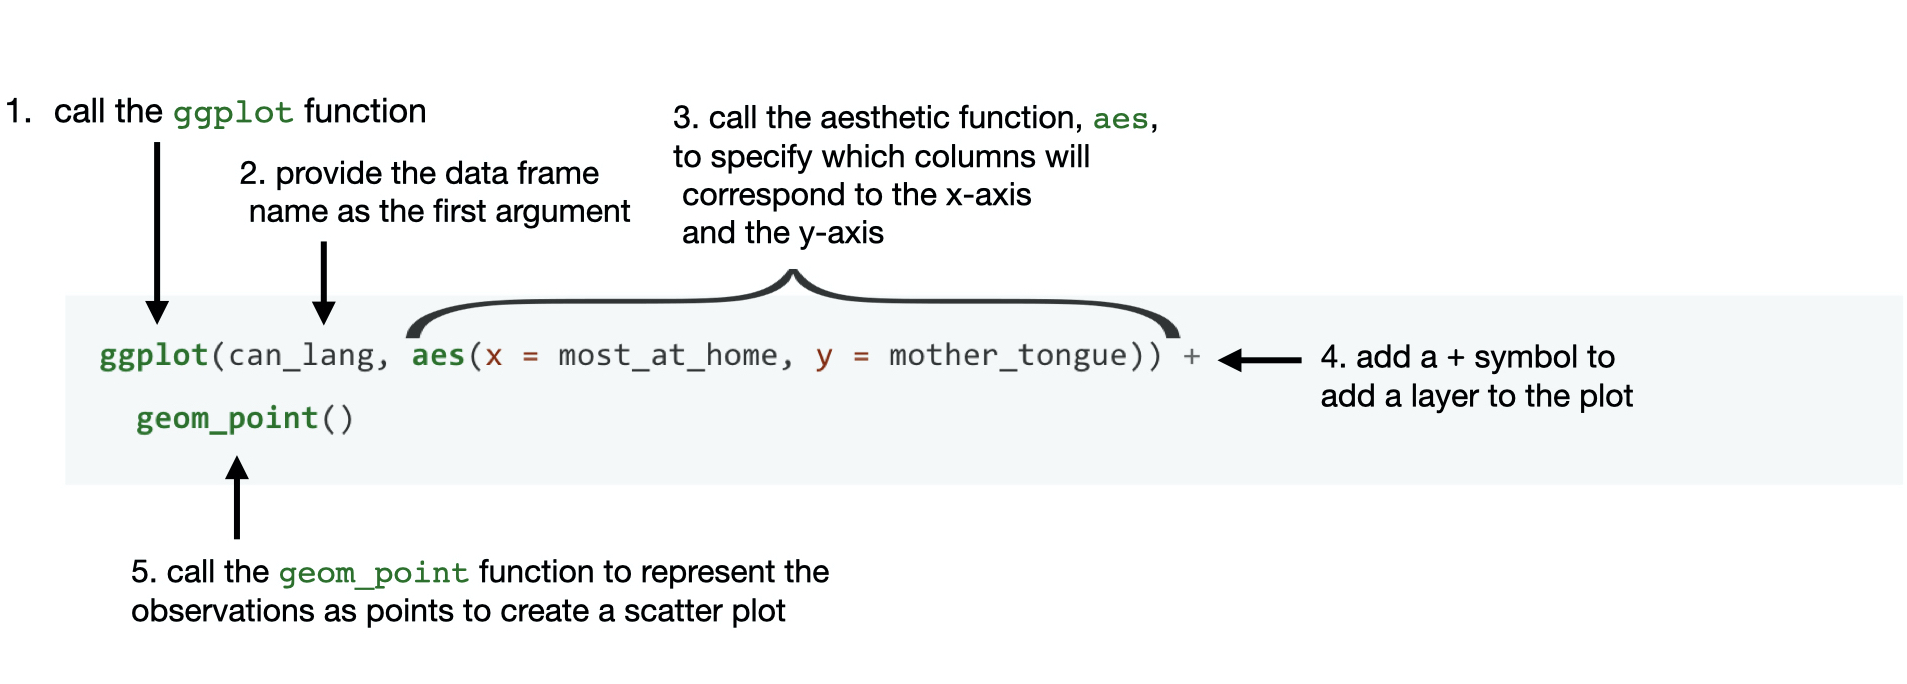
\includegraphics[width=1100pt]{img/ggplot_function} \caption{Creating a bar plot with the ggplot function}\label{fig:img-ggplot}
\end{figure}

\begin{Shaded}
\begin{Highlighting}[]
\FunctionTok{ggplot}\NormalTok{(ten\_lang, }\FunctionTok{aes}\NormalTok{(}\AttributeTok{x =}\NormalTok{ language, }\AttributeTok{y =}\NormalTok{ mother\_tongue)) }\SpecialCharTok{+}
  \FunctionTok{geom\_bar}\NormalTok{(}\AttributeTok{stat =} \StringTok{"identity"}\NormalTok{)}
\end{Highlighting}
\end{Shaded}

\begin{figure}
\centering
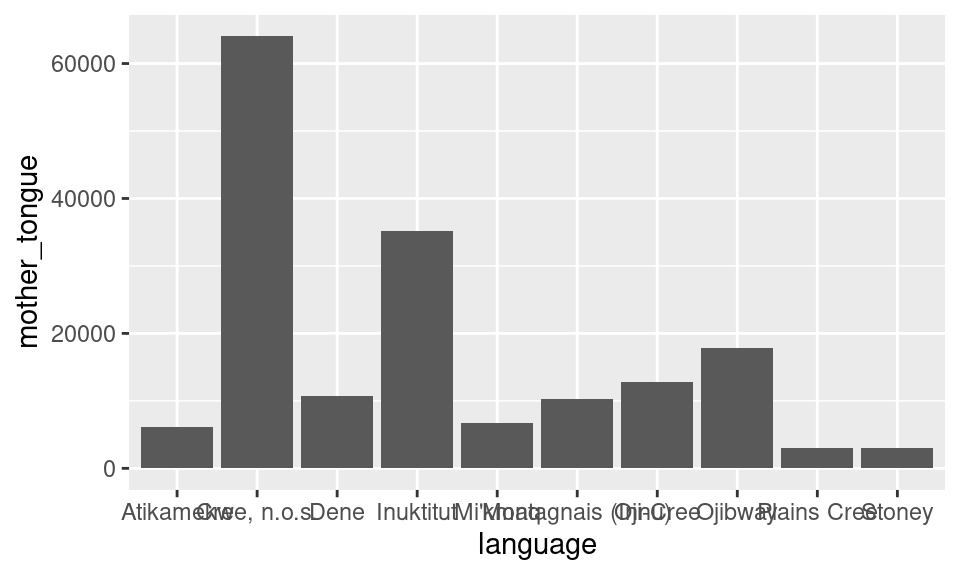
\includegraphics{bookdown_files/figure-latex/barplot-mother-tongue-1.pdf}
\caption{\label{fig:barplot-mother-tongue}Bar plot of the ten Aboriginal languages most often reported by Canadians as their mother tongue}
\end{figure}

\begin{quote}
\textbf{In case you have used R before and are curious:} The vast majority of the
time, a single expression in R must be contained in a single line of code.
However, there \emph{are} a small number of situations in which you can have a
single R expression span multiple lines. Above is one such case: here, R knows that a line cannot
end with a \texttt{+} symbol, \index{plussymb@$+$} and so it keeps reading the next line to figure out
what the right hand side of the \texttt{+} symbol should be. We could, of course,
put all of the added layers on one line of code, but splitting them across
multiple lines helps a lot with code readability. \index{multi-line expression}
\end{quote}

\hypertarget{formatting-ggplot-objects}{%
\subsection{Formatting ggplot objects}\label{formatting-ggplot-objects}}

It is exciting that we can already visualize our data to help answer our
question, but we are not done yet! We can (and should) do more to improve the
interpretability of the data visualization that we created. For example, by
default, R uses the column names as the axis labels. Usually these
column names do not have enough information about the variable in the column.
We really should replace this default with a more informative label. For the
example above, R uses the column name \texttt{mother\_tongue} as the label for the
y axis, but most people will not know what that is. And even if they did, they
will not know how we measure this variable, nor which group of people the
measurements were taken. An axis label that reads ``Mother Tongue (Number of
Canadians, 2016 Census)'' would be much more informative.

Adding additional layers \index{plot!layers} to our visualizations that we create in \texttt{ggplot} is
one common and easy way to improve and refine our data visualizations. New
layers are added to \texttt{ggplot} objects using the \texttt{+} symbol. For example, we can
use the \texttt{xlab} (short for x axis label) and \texttt{ylab} (short for y axis label) functions
to add layers where we specify meaningful
and informative labels for the x and y axes. \index{plot!axis labels} Again, since we are specifying
words (e.g.~\texttt{"Mother\ Tongue\ (Number\ of\ Canadians,\ 2016\ Census)"}) as arguments to
\texttt{xlab} and \texttt{ylab}, we surround them with double-quotes. We can add many more
layers to format the plot further, and we will explore these in Chapter
\ref{viz}.

\begin{Shaded}
\begin{Highlighting}[]
\FunctionTok{ggplot}\NormalTok{(ten\_lang, }\FunctionTok{aes}\NormalTok{(}\AttributeTok{x =}\NormalTok{ language, }\AttributeTok{y =}\NormalTok{ mother\_tongue)) }\SpecialCharTok{+}
  \FunctionTok{geom\_bar}\NormalTok{(}\AttributeTok{stat =} \StringTok{"identity"}\NormalTok{) }\SpecialCharTok{+}
  \FunctionTok{xlab}\NormalTok{(}\StringTok{"Language"}\NormalTok{) }\SpecialCharTok{+}
  \FunctionTok{ylab}\NormalTok{(}\StringTok{"Mother Tongue (Number of Canadians, 2016 Census)"}\NormalTok{)}
\end{Highlighting}
\end{Shaded}

\begin{figure}
\centering
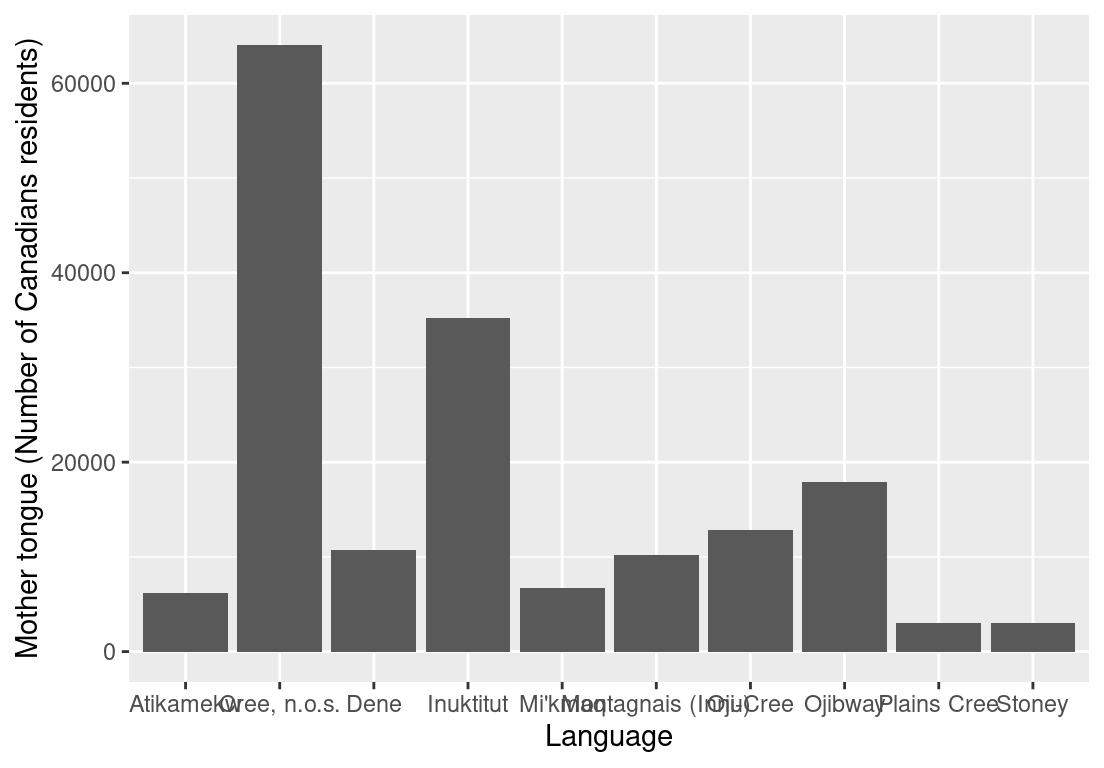
\includegraphics{bookdown_files/figure-latex/barplot-mother-tongue-labs-1.pdf}
\caption{\label{fig:barplot-mother-tongue-labs}Bar plot of the ten Aboriginal languages most often reported by Canadians as their mother tongue with x and y labels}
\end{figure}

The result is shown in Figure \ref{fig:barplot-mother-tongue-labs}.
This is already quite an improvement! Let's tackle the next major issue with the visualization
in Figure \ref{fig:barplot-mother-tongue-labs}: the overlapping x axis labels, which are
currently making it difficult to read the different language names.
One solution is to rotate the plot such that the bars are horizontal rather than vertical.
To accomplish this, we will swap the x and y coordinate axes:

\begin{Shaded}
\begin{Highlighting}[]
\FunctionTok{ggplot}\NormalTok{(ten\_lang, }\FunctionTok{aes}\NormalTok{(}\AttributeTok{x =}\NormalTok{ mother\_tongue, }\AttributeTok{y =}\NormalTok{ language)) }\SpecialCharTok{+}
  \FunctionTok{geom\_bar}\NormalTok{(}\AttributeTok{stat =} \StringTok{"identity"}\NormalTok{) }\SpecialCharTok{+}
  \FunctionTok{xlab}\NormalTok{(}\StringTok{"Mother Tongue (Number of Canadians, 2016 Census)"}\NormalTok{) }\SpecialCharTok{+}
  \FunctionTok{ylab}\NormalTok{(}\StringTok{"Language"}\NormalTok{) }
\end{Highlighting}
\end{Shaded}

\begin{figure}
\centering
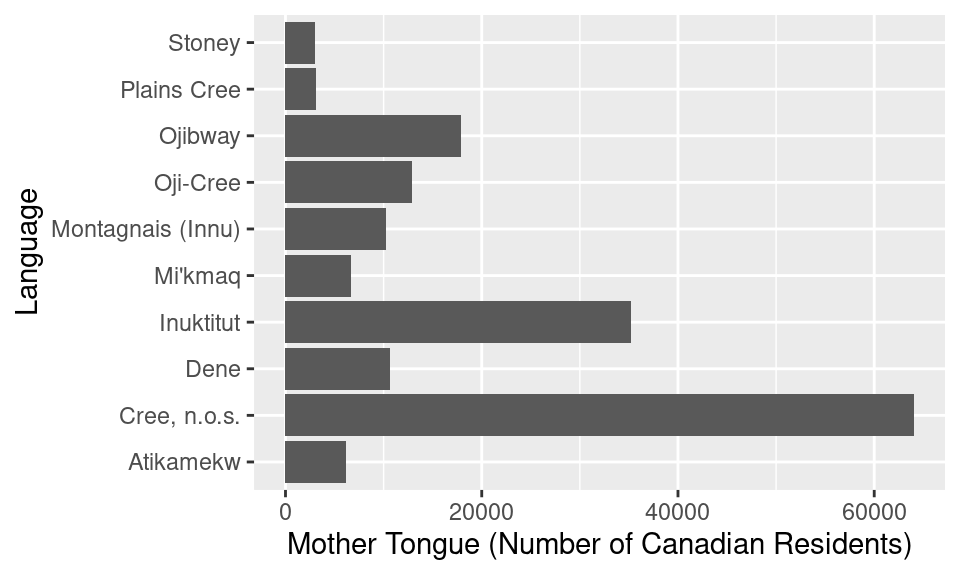
\includegraphics{bookdown_files/figure-latex/barplot-mother-tongue-flipped-1.pdf}
\caption{\label{fig:barplot-mother-tongue-flipped}Horizontal bar plot of the ten Aboriginal languages most often reported by Canadians as their mother tongue}
\end{figure}

Another big step forward, as shown in Figure \ref{fig:barplot-mother-tongue-flipped}! There
are no more serious issues with the visualization. Now comes time to refine
the visualization to make it even more well-suited to answering the question
we asked earlier in this chapter. For example, the visualization could be made more transparent by
organizing the bars according to the number of Canadian residents reporting
each language, rather than in alphabetical order. We can reorder the bars using
the \texttt{reorder} \index{reorder} function, which orders a variable (here \texttt{language}) based on the
values of the second variable (\texttt{mother\_tongue}).

\begin{Shaded}
\begin{Highlighting}[]
\FunctionTok{ggplot}\NormalTok{(ten\_lang, }\FunctionTok{aes}\NormalTok{(}\AttributeTok{x =}\NormalTok{ mother\_tongue, }\AttributeTok{y =} \FunctionTok{reorder}\NormalTok{(language, mother\_tongue))) }\SpecialCharTok{+}
  \FunctionTok{geom\_bar}\NormalTok{(}\AttributeTok{stat =} \StringTok{"identity"}\NormalTok{) }\SpecialCharTok{+}
  \FunctionTok{xlab}\NormalTok{(}\StringTok{"Mother Tongue (Number of Canadians, 2016 Census)"}\NormalTok{) }\SpecialCharTok{+}
    \FunctionTok{ylab}\NormalTok{(}\StringTok{"Language"}\NormalTok{) }
\end{Highlighting}
\end{Shaded}

\begin{figure}
\centering
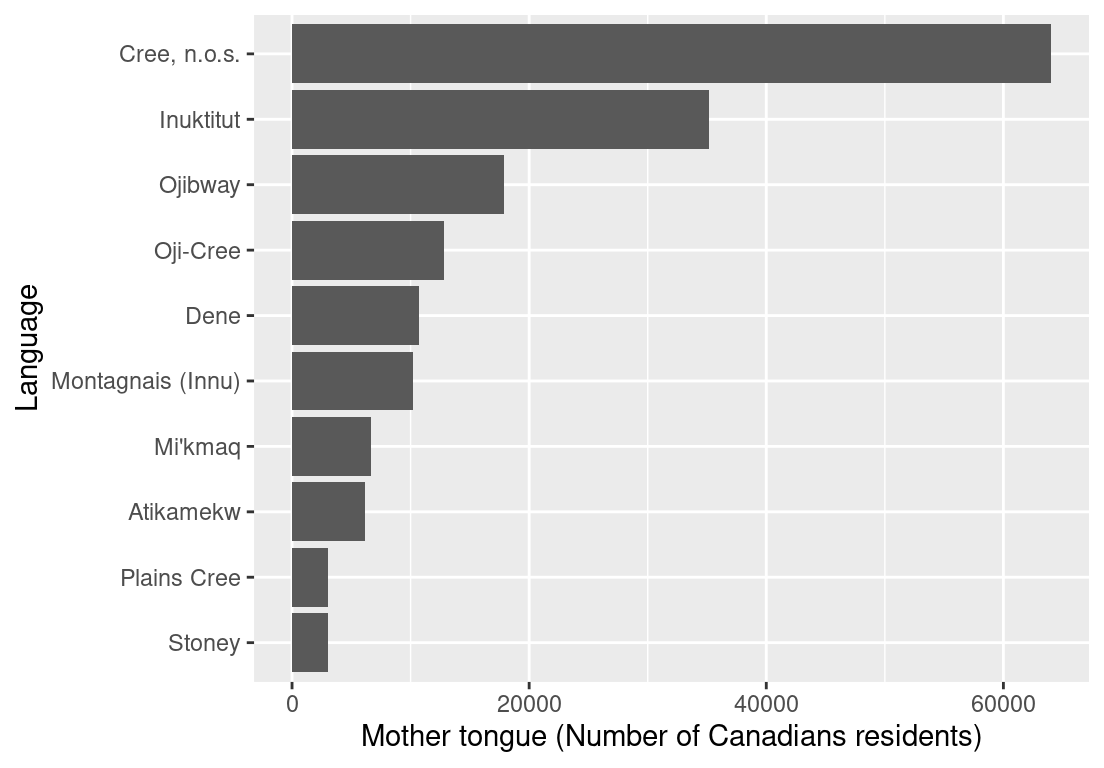
\includegraphics{bookdown_files/figure-latex/barplot-mother-tongue-reorder-1.pdf}
\caption{\label{fig:barplot-mother-tongue-reorder}Bar plot of the ten Aboriginal languages most often reported by Canadians as their mother tongue with bars reordered}
\end{figure}

Figure \ref{fig:barplot-mother-tongue-reorder} provides a very clear and well-organized
answer to our original question; we can see what the ten most often reported Aboriginal languages
were, according to the 2016 Candian census, and how many people speak each of them. For
instance, we can see that the Aboriginal language most often reported was Cree
n.o.s. with over 60,000 Canadian residents reporting it as their mother tongue.

\begin{quote}
``n.o.s.'' means ``not otherwise specified'', so Cree n.o.s. refers to
individuals who reported Cree as their mother tongue. In this data set, the
Cree languages include the following categories: Cree n.o.s., Swampy Cree,
Plains Cree, Woods Cree, and a `Cree not included elsewhere' category (which
includes Moose Cree, Northern East Cree and Southern East Cree)
\citep{language2018}.
\end{quote}

\hypertarget{putting-it-all-together}{%
\subsection{Putting it all together}\label{putting-it-all-together}}

In the block of code below, we put everything from this chapter together, with a few
modifications. In particular, we have
added a few more layers to make the data visualization even more effective.
Specifically, we changed the colour of the bars and changed the background from
grey to white to improve the contrast. We have also actually skipped the
\texttt{select} step that we did above; since you specify the variable names to plot
in the \texttt{ggplot} function, you don't actually need to \texttt{select} the columns in advance
when creating a visualization. And finally, we provided \emph{comments} next to
many of the lines of code below using the
hash symbol \texttt{\#}. When R sees a \texttt{\#} sign, \index{comment} \index{commentsymb@\#|see{comment}} it
will ignore all of the text that
comes after the symbol on that line. So you can use comments to explain lines
of code for others, and perhaps more importantly, your future self!
It's good practice to get in the habit of
commenting your code to improve its readability.

\begin{Shaded}
\begin{Highlighting}[]
\FunctionTok{library}\NormalTok{(tidyverse)}

\CommentTok{\# load the data set}
\NormalTok{can\_lang }\OtherTok{\textless{}{-}} \FunctionTok{read\_csv}\NormalTok{(}\StringTok{"data/can\_lang.csv"}\NormalTok{)}

\CommentTok{\# obtain the 10 most common Aboriginal languages}
\NormalTok{aboriginal\_lang }\OtherTok{\textless{}{-}} \FunctionTok{filter}\NormalTok{(can\_lang, category }\SpecialCharTok{==} \StringTok{"Aboriginal languages"}\NormalTok{)}
\NormalTok{arranged\_lang }\OtherTok{\textless{}{-}} \FunctionTok{arrange}\NormalTok{(aboriginal\_lang, }\AttributeTok{by =} \FunctionTok{desc}\NormalTok{(mother\_tongue))}
\NormalTok{ten\_lang }\OtherTok{\textless{}{-}} \FunctionTok{slice}\NormalTok{(arranged\_lang, }\DecValTok{1}\SpecialCharTok{:}\DecValTok{10}\NormalTok{)}

\CommentTok{\# create the visualization}
\FunctionTok{ggplot}\NormalTok{(ten\_lang, }\FunctionTok{aes}\NormalTok{(}
  \AttributeTok{x =}\NormalTok{ mother\_tongue,}
  \AttributeTok{y =} \FunctionTok{reorder}\NormalTok{(language, mother\_tongue)  }\CommentTok{\# make sure the plot orders the bars by size}
\NormalTok{)) }\SpecialCharTok{+}
  \FunctionTok{geom\_bar}\NormalTok{(}\AttributeTok{stat =} \StringTok{"identity"}\NormalTok{, }\AttributeTok{fill =} \StringTok{"steelblue"}\NormalTok{) }\SpecialCharTok{+}
  \FunctionTok{xlab}\NormalTok{(}\StringTok{"Mother Tongue (Number of Canadians, 2016 Census)"}\NormalTok{) }\SpecialCharTok{+}
  \FunctionTok{ylab}\NormalTok{(}\StringTok{"Language"}\NormalTok{) }\SpecialCharTok{+}
  \FunctionTok{theme\_bw}\NormalTok{() }\CommentTok{\# use a theme to have a white background}
\end{Highlighting}
\end{Shaded}

\begin{figure}
\centering
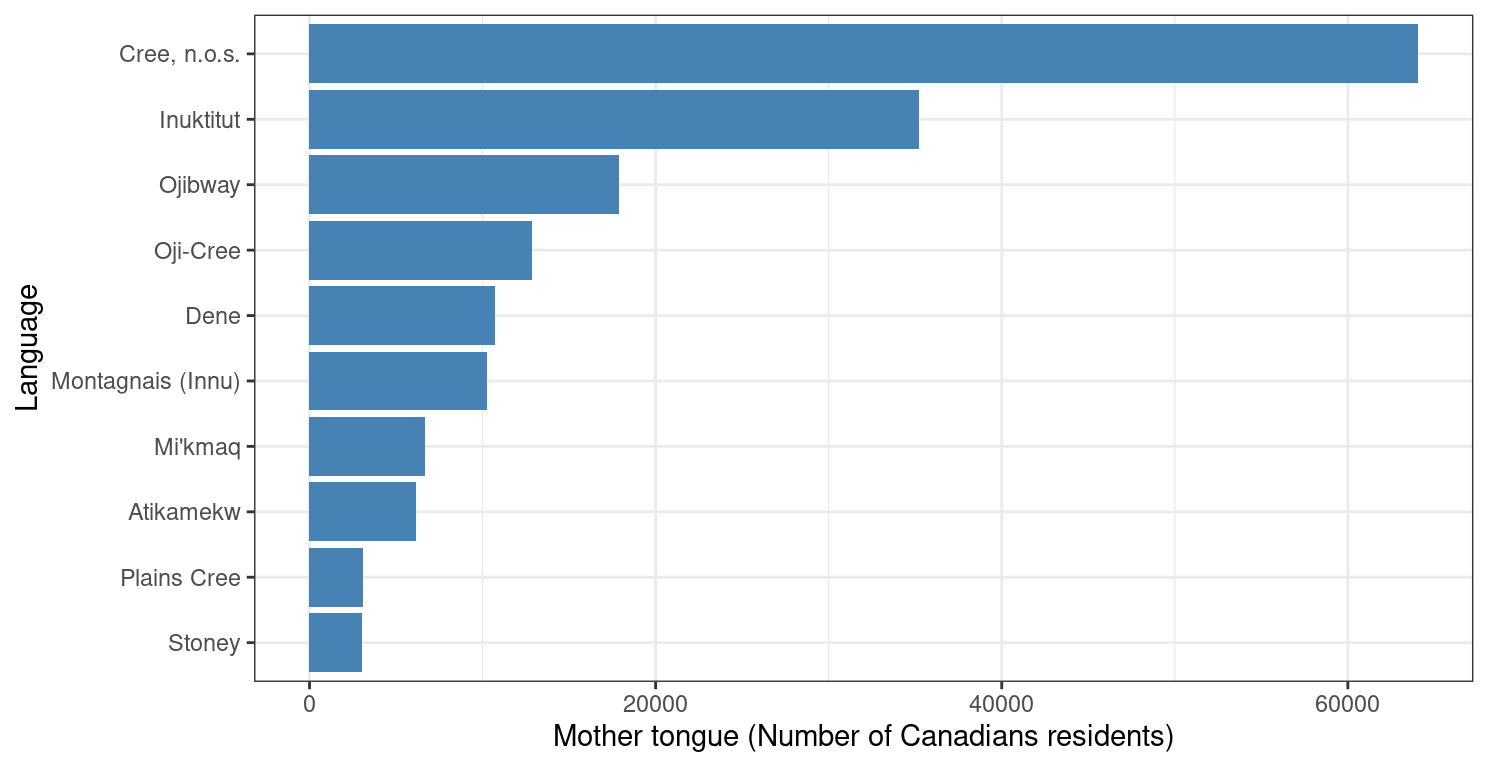
\includegraphics{bookdown_files/figure-latex/nachos-to-cheesecake-1.pdf}
\caption{\label{fig:nachos-to-cheesecake}Putting it all together: bar plot of the ten Aboriginal languages most often reported by Canadians as their mother tongue}
\end{figure}

This exercise demonstrates the power of R. In relatively few lines of code, we
performed an entire data science workflow with a highly effective data
visualization! We asked a question, loaded the data into R, wrangled the data
(using \texttt{filter}, \texttt{arrange} and \texttt{slice}) and created a data visualization to
help answer our question. In this chapter, you got a quick taste of the data
science workflow; continue on with the next few chapters to learn each of
these steps in much more detail!

\hypertarget{accessing-documentation}{%
\section{Accessing documentation}\label{accessing-documentation}}

There are many R functions in the \texttt{tidyverse} package (and beyond!), and
nobody can be expected to remember what every one of them does
nor all of the arguments we have to give them. Fortunately R provides
the \texttt{?} symbol, which
\index{questionmark@? symbol|see{documentation}}
\index{help|see{documentation}}
\index{documentation} provides an easy way to pull up the documentation for
most functions quickly. To use the \texttt{?} symbol to access documentation, you
just put the name of the function you are curious about after the \texttt{?} symbol.
For example, if you had forgotten what the \texttt{filter} function
did or exactly what arguments to pass in, you could run the following
code:

\begin{verbatim}
?filter
\end{verbatim}

Figure \ref{fig:01-help} shows the documentation that will pop up,
including a high-level description of the function, its arguments,
a description of each, and more. Note that you may find some of the
text in the documentation a bit too technical right now
(for example, what is \texttt{dbplyr}, and what is grouped data?).
Fear not: as you work through this book, many of these terms will be introduced
to you, and slowly but surely you will become more adept at understanding and navigating
documentation like that shown in Figure \ref{fig:01-help}. But do keep in mind that the documentation
is not written to \emph{teach} you about a function; it is just there as a reference to \emph{remind}
you about the different arguments and usage of functions that you have already learned about elsewhere.
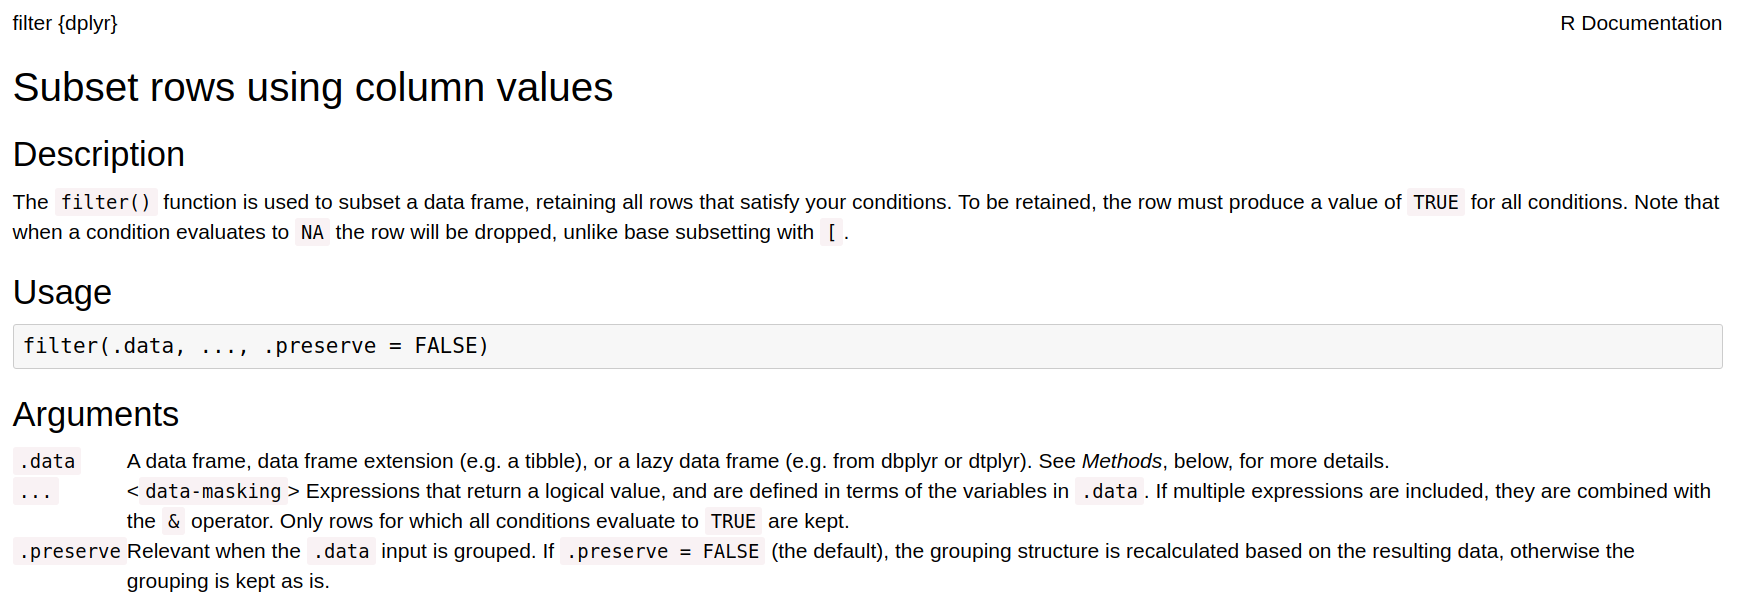
\includegraphics{img/help-filter.png}

  \bibliography{references.bib}

\printindex

\end{document}
